\documentclass[fr,license=none]{../../../eplsummary}

\usepackage{graphicx}

\usepackage[SIunits]{../../../eplunits}

\newcommand\fv[1]{\textbf{#1}} % vector
\newcommand\vp[2]{#1 \wedge #2} % vector product
\renewcommand\sp[2]{#1 \cdot #2} % scalar product
\newcommand\rot[1]{\vp{\grad{}}{#1}} % vector product
\renewcommand\div[1]{\sp{\grad{}}{#1}} % vector product

\DeclareMathOperator{\trace}{tr}
\DeclareMathOperator{\cof}{cof}
\DeclareMathOperator{\mydiv}{div}
\DeclareMathOperator{\mygrad}{grad}
\DeclareMathOperator{\myrot}{rot}

\hypertitle{Mécanique des milieux continus}{5}{MECA}{1901}
{Laurent Opsomer}
{Philippe Chatelain et Emilie Marchandise}

\part*{Introduction}
Un milieu continu est un milieu pour lequel on a fait l'hypothèse que la matière est distribuée continûment (on ne tient pas compte de la structure moléculaire par exemple). Dans un tel milieu, toutes les quantités physiques telles que la masse volumique, les déplacements, les vitesses, les contraintes etc., varient de manière continue. Leurs dérivées spatiales sont donc bien définies.
\paragraph{}
Pour étudier un point matériel ou une particule, on regarde un volume infinitésimal $\Delta V$, le Volume \'Elémentaire Représentatif (VER), sous l'hypothèse $$\lambda \ll L_{VER} \ll L$$

\part{Vecteurs et tenseurs}
\section{Algèbre vectoriel}
\subsection{Produit scalaire}

\[ \sp{\fv{F}}{\fv{d}} = Fd\cos\theta \qquad 0\leq \theta \leq \pi. \]
Le produit scalaire est commutatif et distributif. La projection orthogonale d'un vecteur \fv{A} le long d'une direction \fv{ê} est donnée par
$(\sp{\fv{A}}{\fv{ê}})\fv{ê}$.

\subsection{Produit vectoriel}
\[ \fv{C} = \vp{\fv{A}}{\fv{B}}=AB\sin(\fv{A},\fv{B})\fv{ê}
= AB\sin\theta\hspace{0.1cm}\fv{ê}. \]
\paragraph{}
La norme de \fv{C} est l'aire du parallélogramme représenté par les vecteurs \fv{A} et \fv{B}.
\paragraph{}
Le produit vectoriel n'est pas commutatif: $\vp{\fv{A}}{\fv{B}} = -\vp{\fv{B}}{\fv{A}}$. En revanche, il est distributif (mais l'ordre des facteurs doit être maintenu).

\subsection{Produits triples de vecteurs}
\begin{itemize}
  \item Produit mixte: $\sp{\fv{A}}{(\vp{\fv{B}}{\fv{C}})}$ représente le volume du parallélépipède formé par les vecteurs \fv{A}, \fv{B} et \fv{C}. Condition nécessaire et suffisante pour que 3 vecteurs soient coplanaires: $\fv{A}\cdot(\fv{B}\wedge\fv{C})=0$
  \item $\fv{A}\cdot\fv{B}\wedge\fv{C}=\fv{A}\wedge\fv{B}\cdot\fv{C}\equiv[\fv{ABC}]$
  \item $\fv{A}\cdot \fv{B}\wedge\fv{C} = \fv{C}\cdot\fv{A}\wedge\fv{B}=\fv{B}\cdot\fv{C}\wedge\fv{A}\equiv[\fv{ABC}]$
  \item $\fv{A}\cdot \fv{B}\wedge\fv{C} = -\fv{A}\cdot\fv{C}\wedge\fv{B}=-\fv{B}\cdot\fv{A}\wedge\fv{C}$
  \item Double produit vectoriel: $\fv{A}\wedge(\fv{B}\wedge\fv{C})=(\fv{A}\cdot\fv{C})\fv{B}-(\fv{A}\cdot\fv{B})\fv{C}$: vecteur perpendiculaire à \fv{A} et situé dans le plan formé par \fv{B} et \fv{C}. (Notation indicielle: $e_{ijk}e_{klm}A_jB_lC_m\fv{ê}_i$)
\end{itemize}

\subsection{Composantes d'un vecteur}

Soient $\fv{A}=A_1\fv{ê}_1+A_2\fv{ê}_2+A_3\fv{ê}_3$ et $\fv{B}=B_1\fv{ê}_1+B_2\fv{ê}_2+B_3\fv{ê}_3$. On a:
$$\begin{array}{r l}
\fv{A}\cdot\fv{B} =&(A_1 \fv{ê}_1+A_2\fv{ê}_2+A_3\fv{ê}_3)\cdot(B_1\fv{ê}_1+B_2\fv{ê}_2+B_3\fv{ê}_3)\\
 =&A_1B_1 + A_2B_2+A_3B_3\\
\fv{A}\wedge\fv{B}=&(A_1 \fv{ê}_1+A_2\fv{ê}_2+A_3\fv{ê}_3)\wedge(B_1\fv{ê}_1+B_2\fv{ê}_2+B_3\fv{ê}_3)\\
 =&(A_2B_3-A_3B_2)\fv{ê}_1+(A_3B1-A1B_3)\fv{ê}_2+(A_1B_2-A_2B_1)\fv{ê}_3\\
\end{array}$$

\section{Notation indicielle et convention de sommation}
\paragraph{Convention de sommation (Einstein):} $$\sum_{i=1}^3 A_i\fv{e}_i \equiv A_i\fv{e}_i$$
\paragraph{Indice muet:} indice répété qui peut être remplacé par n'importe quel indice qui n'a pas encore été utilisé. Il indique qu'une somme doit être effectuée sur toutes les valeurs possibles. Par exemple: $$\fv{A}=A_i\fv{e}_i=A_j\fv{e}_j$$
Aucun indice ne peut apparaître plus de deux fois dans une expression.
\paragraph{Indice libre:} indice qui apparaît dans chaque expression d'une équation (à l'exception de celles qui ne contiennent que des scalaires), une seule fois dans chaque terme. Par exemple, l'indice $k$ dans $G_k = H_k(2-3A_iB_i)+P_jQ_jF_k$

\section{Symboles de Kronecker et de Levi-Civita}

\subsection{Symbole de Kronecker:} $\fv{ê}_i\cdot\fv{ê}_j=\delta_{ij}$

avec $\delta_{ij}=\left\{
	\begin{array}{l c c}
		1, & \text{si} & i=j\\
		0, & \text{si} & i\neq j\\
	\end{array}\right.$
\paragraph{} On a ainsi: $$A_i\delta_{ij}=A_j, \qquad A_iB_j\delta_{ij}=A_iB_i=A_jB_j, \qquad \delta_{ij}\delta_{ik}=\delta_{jk}$$

\paragraph{} Le produit scalaire peut être exprimé en notation indicielle, dans une base orthonormale, en utilisant le symbole de Kronecker: $\fv{A}\cdot\fv{B}=(A_i\fv{ê}_i)\cdot(B_j\fv{ê}_j) = A_iB_j\delta_{ij}=A_iB_i$

\subsection{Symbole de Levi-Civita (ou de permutation):}
$$e_{ijk}=\left\{
\begin{array}{r l}
	1, & \text{si }i,j,k \text{ sont dans l'ordre cyclique et }i\neq j\neq k\\
	-1, & \text{si }i,j,k \text{ ne sont pas dans l'ordre cyclique et } i\neq j\neq k\\
	0, & \text{si l'un des indices est répétés}
\end{array} \right.$$
\paragraph{}
On écrit par définition pour le produit vectoriel $\fv{ê}_i\wedge\fv{ê}_j$: $$\fv{ê}_i\wedge\fv{ê}_j\equiv e_{ijk}\fv{ê}_k\hspace{0.3cm} \text{ou} \hspace{0.3cm} e_{ijk}=\fv{ê}_i\wedge \fv{ê}_j \cdot \fv{ê}_k=\fv{ê}_i\cdot \fv{ê}_j \wedge \fv{ê}_k$$
\paragraph{}
Vu la définition, on a également $e_{ijk} = e_{kij} = e_{jki} = -e_{jik} \text{ etc.}$
\paragraph{}Le produit vectoriel peut être exprimé en notation indicielle, dans une base orthonormale, en utilisant le symbole de permutation: $\fv{A}\wedge\fv{B}=(A_i\fv{ê}_i)\wedge(B_j\fv{ê}_j) = A_iB_je_{ijk}\fv{ê}_k$. Pour le produit mixte on a: $\fv{u}\cdot(\fv{v}\wedge\fv{w})=e_{ijk}u_iv_jw_k$
\paragraph{} Le symbole de Kronecker et le symbole de Levi-Civita sont reliés par l'identité:
$$e_{ijk}e_{imn}=\delta_{jm}\delta_{kn}-\delta_{jn}\delta_{km}$$

\paragraph{Remarque:} Toute écriture vectorielle de toute identité est \emph{invariante}, c'est-à-dire valide dans la base orthonormée associée à n'importe quel système de coordonnées.

\section{Loi de transformation}
Soient $\{\fv{ê}_1, \fv{ê}_2, \fv{ê}_3\}$ et $\{\hat{\bar{\fv{e}}}_1, \hat{\bar{\fv{e}}}_2, \hat{\bar{\fv{e}}}_3\}$ deux bases orthonormales distinctes. On peut exprimer le même vecteur dans les deux bases:
$$\begin{array}{c c c c c}
\fv{A} &=& A_i\fv{ê}_i &=& (\fv{A}\cdot \fv{ê}_i)\fv{ê}_i\\
 &=& \bar{A}_i\hat{\bar{\fv{e}}}_i &=& (\fv{A}\cdot \hat{\bar{\fv{e}}}_i)\hat{\bar{\fv{e}}}_i\\
\end{array}$$
d'où:  $$\bar{A}_j=\fv{A}\cdot\hat{\bar{\fv{e}}}_j=(A_i\fv{ê}_i)\cdot\hat{\bar{\fv{e}}}_j=A_i(\fv{ê}_i\cdot\hat{\bar{\fv{e}}}_j)\equiv l_{ij}A_i$$
Cette équation est la loi de transformation entre les composantes avec barre et sans barre. Les coefficients $l_{ij}$ sont les cosinus directeurs des angles entre $\hat{\bar{\fv{e}}}_i$ et $\fv{ê}_j$. Nous pouvons les regrouper dans la matrice \fv{L} de la transformation:

$$\fv{L}= \left[
\begin{array}{c c c}
l_{11}& l_{12}& l_{13} \\
l_{21}& l_{22}& l_{23}\\
l_{31}& l_{32}& l_{33}\\
\end{array}\right]$$
Ce qui permet d'écrire:
$$\left\{
\begin{array}{c}
\bar{A}_1\\
\bar{A}_2\\
\bar{A}_3
\end{array}\right\} = \fv{L} \left\{\begin{array}{c}
A_1\\
A_2\\
A_3\\
\end{array}\right\}$$

\section{Théorie des matrices}
\subsection{Quelques propriétés importantes (rappels): }
\begin{itemize}
\item Un matrice carrée \fv{A} est dite \emph{normale} si $\fv{A}\fv{A}^T=\fv{A}^T\fv{A}$. Elle est \emph{orthogonale} si de plus $\fv{A}^T\fv{A}=I$ ($\fv{A}=\fv{A}^{-1})$
\item La multiplication de matrices est associative
\item S'il existe, l'inverse d'une matrice \fv{A} est unique. Si \fv{A} n'est pas inversible, elle est dite \emph{singulière}.
\item $\det(\fv{AB})=\det\fv{A}\cdot\det\fv{B}$
\item $\det \fv{A}^T=\det\fv{A}$
\item $\det(\alpha\fv{A})=\alpha^n\det\fv{A}$, $n$ étant l'ordre de \fv{A}
\item $\fv{A}^{-1}=\frac{1}{\det\fv{A}}(\cof(\fv{A}))^T$
\end{itemize}
\paragraph*{}
Le produit vectoriel de deux vecteurs peut être exprimé par le déterminant
$$\fv{A}\wedge\fv{B}\equiv
\begin{vmatrix}
\fv{ê}_1 & \fv{ê}_2 &\fv{ê}_3\\
A_1 & A_2 &	 A_3\\
B_1 & B_2 & B_3\\
\end{vmatrix}$$
alors que le produit mixte s'écrit
$$\fv{C}\cdot(\fv{A}\wedge\fv{B})\equiv
\begin{vmatrix}
  C_1&C_2&C_3\\
  A_1&A_2&A_3\\
  B_1&B_2&B_3\\
\end{vmatrix}.$$

\section{Calcul vectoriel}
\subsection{Opérateur nabla}
L'opérateur nabla ($\nabla$) est utilisé pour exprimer le gradient d'une fonction: $$\nabla\phi\equiv\mygrad(\phi)=\fpart{\phi}{\fv{x}}$$ Le vecteur $\fpart{\phi}{\fv{x}}$ peut être interprété comme étant égal à l'action d'un opérateur (l'\emph{opérateur nabla}) sur la fonction $\phi$:
$$\nabla\equiv \fv{ê}_i\fpart{}{x_i}$$
Attention cependant, cet opérateur ne possède pas toutes les propriétés d'un vecteur! Par exemple, $\nabla\cdot\fv{A}\neq\fv{A}\cdot\nabla$.
\paragraph{}
On peut utiliser le gradient pour calculer la \emph{dérivée directionnelle} d'un champ scalaire $\phi=\phi(x)$.
La dérivée dans la direction $\fv{ê}$ de $\phi$ est $$\left(\fdif{\phi}{s}\right)_{\fv{ê}}=\fdif{\fv{x}}{s}\cdot\nabla\phi=\fv{ê}\cdot\nabla\phi$$

\subsection{Divergence et rotationnel d'un vecteur}
La \emph{divergence} d'un vecteur est définie comme suit:
\[ \mydiv\fv{A} \equiv \div \fv{A}=\fpart{A_1}{x_1}+\fpart{A_2}{x_2}+\fpart{A_3}{x_3} \]
La divergence du gradient d'une fonction est appelée le \emph{laplacien}: $$\mydiv(\mygrad(\phi))\equiv \nabla^2\phi=\frac{\partial^2\phi}{\partial x_i\partial x_i}$$
\paragraph{}
Le \emph{rotationnel} d'un vecteur est défini comme:
$$\myrot\fv{A}=\rot \fv{A}=e_{ijk}\fv{ê}_i\fpart{A_k}{x_j}$$

\subsection{Coordonnées cylindriques et sphériques}
\paragraph{Système de coordonnées cylindriques}
$$\left\{\begin{array}{c}
\fv{ê}_r\\
\fv{ê}_{\theta}\\
\fv{ê}_z
\end{array}\right\}=
\left[\begin{array}{ccc}
\cos\theta&\sin\theta&0\\
-\sin\theta&\cos\theta&0\\
0&0&1
\end{array}\right]
\left\{\begin{array}{c}
\fv{ê}_x\\
\fv{ê}_y\\
\fv{ê}_z
\end{array}\right\}$$

$$\left\{\begin{array}{c}
\fv{ê}_x\\
\fv{ê}_{y}\\
\fv{ê}_z
\end{array}\right\}=
\left[\begin{array}{ccc}
\cos\theta&-\sin\theta&0\\
\sin\theta&\cos\theta&0\\
0&0&1
\end{array}\right]
\left\{\begin{array}{c}
\fv{ê}_r\\
\fv{ê}_{\theta}\\
\fv{ê}_z
\end{array}\right\}$$

\paragraph{Système de coordonnées sphériques}
$$\left\{\begin{array}{c}
\fv{ê}_R\\
\fv{ê}_{\phi}\\
\fv{ê}_{\theta}
\end{array}\right\}=
\left[\begin{array}{ccc}
\cos\theta\sin\phi&\sin\theta\sin\phi&\cos\phi\\
\cos\theta\cos\phi&\cos\phi\sin\theta&-\sin\phi\\
-\sin\theta&\cos\theta&0
\end{array}\right]
\left\{\begin{array}{c}
\fv{ê}_x\\
\fv{ê}_y\\
\fv{ê}_z
\end{array}\right\}$$

$$\left\{\begin{array}{c}
\fv{ê}_x\\
\fv{ê}_{y}\\
\fv{ê}_z
\end{array}\right\}=
\left[\begin{array}{ccc}
\cos\theta\sin\phi&\cos\phi\cos\theta&-sin\theta\\
\sin\theta\sin\phi&\cos\phi\sin\theta&\cos\theta\\
\cos\phi&-\sin\phi&0
\end{array}\right]
\left\{\begin{array}{c}
\fv{ê}_R\\
\fv{ê}_{\phi}\\
\fv{ê}_{\theta}
\end{array}\right\}$$

(Le tableau 2.6.2 page 51 du livre donne les vecteurs de base et opérateurs différentiels vectoriels dans les systèmes de coordonnées cylindrique et sphérique avec base orthonormée).

\subsection{Théorèmes du gradient, de Green-Ostrogradski et du rotationnel}

Considérons une région $\Omega$ de $\R^3$ délimitée par la surface fermée $\partial \Omega$.
Soient $\dif s$ un élément différentiel de surface,
\fv{\^{n}} la normale unitaire sortante et $\dif v$ un élément de volume infinitésimal de $\Omega$.
$\sp{\fv{A}}{\fv{\^n}} \dif s$ est le \emph{flux} de \fv{A} à travers la surface infinitésimal $\dif s$.
Son intégrale est le flux total au travers de la frontière $\Delta s=\partial\Omega$.

\paragraph*{Théorème du gradient:} $$\int_{\Omega}\nabla\phi \dif v=\oint_{\partial\Omega}\fv{\^n}\,\phi\dif s=\oint_{\partial\Omega}\phi\dif \fv{s}$$
Ce théorème met en relation l'intégrale de volume du gradient d'un champ scalaire et l'intégrale de surface du même champ.
\paragraph*{Théorème de Green-Ostrogradski ou de la divergence:}
$$\int_{\Omega}\nabla\cdot\fv{A}\dif v=\oint_{\partial\Omega}\fv{\^n}\cdot \fv{A}\dif s$$
Ce théorème montre l'égalité entre l'intégrale de la divergence d'un champ vectoriel sur un volume dans $\R^3$ et le flux de ce champ à travers la frontière du volume (qui est une intégrale de surface).
\paragraph*{Théorème du rotationnel: }
$$\int_{\Omega}\nabla\wedge\fv{A}\dif v=\oint_{\partial\Omega}\fv{\^n}\wedge\fv{A}\dif s$$
Ce théorème met en relation l'intégrale de volume du rotationnel d'un champ vectoriel à l'intégrale de surface du même champ.
\paragraph{}
Ces trois théorèmes restent valables dans le cas où \fv{A} est un tenseur et $\phi$ une fonction vectorielle (mais attention à l'ordre des opérations).

\section{Tenseurs}
Un tenseur est une application multilinéaire. Les tenseurs sont des objets plus généraux que les vecteurs, ils sont dotés d'une amplitude et de plusieurs directions mais vérifient les règles d'addition vectorielle et de multiplication scalaire. Les scalaires sont des tenseurs d'ordre 0 et les vecteurs des tenseurs d'ordre 1.
\subsection{Tenseurs dyadiques}
Des quantités qui nécessitent deux directions pour être spécifiées sont des \emph{dyades}, ou \textit{tenseurs du deuxième ordre}. Un tenseur du deuxième ordre est défini comme deux vecteurs localisés au même point et agissant comme une seule entité. Un \emph{tenseur dyadique} est un tenseur du deuxième ordre particulier, formé en juxtaposant des paires de vecteurs, c'est-à-dire en faisant une combinaison linéaire de dyades. En trois dimensions cela donne par exemple, pour des vecteurs \fv{A} et \fv{B}:
\begin{equation*}
\begin{array}{cc}
\mathbf{\Phi}=\fv{A}\fv{B}\equiv\fv{A}\otimes\fv{B}=&A_1B_1\fv{ê}_1\fv{ê}_1+A_1B_2\fv{ê}_1\fv{ê}_2+A_1B_3\fv{ê}_1\fv{ê}_3\\
 &+A_2B_1\fv{ê}_2\fv{ê}_1+A_2B_2\fv{ê}_2\fv{ê}_2+A_2B_3\fv{ê}_2\fv{ê}_3\\
 &+A_3B_1\fv{ê}_3\fv{ê}_1+A_3B_2\fv{ê}_3\fv{ê}_2+A_3B_3\fv{ê}_3\fv{ê}_3\\
\end{array}
\end{equation*}
Nous avons donc $$\begin{array}{cc}
\mathbf{\Phi}=&\phi_{11}\fv{ê}_1\fv{ê}_1+\phi_{12}\fv{ê}_1\fv{ê}_2+\phi_{13}\fv{ê}_1\fv{ê}_3\\
 &+\phi_{21}\fv{ê}_2\fv{ê}_1+\phi_{22}\fv{ê}_2\fv{ê}_2+\phi_{23}\fv{ê}_2\fv{ê}_3\\
 &+\phi_{31}\fv{ê}_3\fv{ê}_1+\phi_{32}\fv{ê}_3\fv{ê}_2+\phi_{33}\fv{ê}_3\fv{ê}_3\\
\end{array}$$
Un tenseur dyadique défini dans un espace tridimensionnel possède ainsi 9 composantes indépendantes, chacune étant associée à une certaine paire de dyades. On peut représenter le tenseur dyadique sous forme d'une matrice:
$$[\mathbf{\Phi}]=\left[\begin{array}{ccc}
\phi_{11}&\phi_{12}&\phi_{13}\\
\phi_{21}&\phi_{22}&\phi_{23}\\
\phi_{31}&\phi_{32}&\phi_{33}
\end{array}\right]\Rightarrow \mathbf{\Phi}=\left\{\begin{array}{c}
\fv{ê}_1\\
\fv{ê}_2\\
\fv{ê}_3\\
\end{array}\right\}^T [\mathbf{\Phi}]\left\{
\begin{array}{c}
\fv{ê}_1\\
\fv{ê}_2\\
\fv{ê}_3\\
\end{array}\right\} $$
\paragraph{}
Le produit scalaire d'un tenseur dyadique avec un vecteur \fv{V} est défini comme suit:
$$\mathbf{\Phi}\cdot\fv{V} = \fv{A}(\fv{B}\cdot\fv{V})=\fv{V}\cdot\mathbf{\Phi}^T$$
$$\fv{V}\cdot\mathbf{\Phi} = (\fv{V}\cdot\fv{A})\fv{B}=\mathbf{\Phi}^T\cdot\fv{V}$$
Le produit scalaire d'un tenseur dyadique avec un vecteur donne donc un vecteur. La transposée du produit de tenseurs suit la règle $$(\mathbf{\Psi}\cdot\mathbf{\Phi})^T=\mathbf{\Phi}^T\cdot\mathbf{\Psi}^T$$
\paragraph{}
Le tenseur unité est défini par $\fv{I}=\delta_{ij}\fv{ê}_i\fv{ê}_j=\fv{ê}_i\fv{ê}_i$ (symétrique) $\Rightarrow [\fv{I}]=\left[\begin{array}{ccc}
1&0&0\\
0&1&0 \\
0&0&1
\end{array}\right]$
\paragraph{}
Le \emph{double produit contracté} (commutatif) est le scalaire $$(\fv{AB}):(\fv{CD})\equiv (\fv{B}\cdot\fv{C})(\fv{A}\cdot\fv{D}).$$
Dans une base cartésienne cela donne, pour deux tenseurs du deuxième ordre:
$$\mathbf{\Phi}:\mathbf{\Psi}=(\phi_{ij}\fv{ê}_i\fv{ê}_j):(\psi_{mn}\fv{ê}_m\fv{ê}_n)=\phi_{ij}\psi_{ji}$$
On peut aussi calculer le double produit contracté via la notation matricielle:
$$[\mathbf{\Psi}:\mathbf{\Phi}]=\trace([\mathbf{\Psi}][\mathbf{\Phi}]).$$

\subsection{Transformation des composantes d'une dyade}
Exprimons $\mathbf{\Phi}$ dans deux bases cartésiennes différentes: $$\mathbf{\Phi}=\phi_{ij}\fv{ê}_i\fv{ê}_j=\bar{\phi}_{kl}\mathbf{\hat{\bar{e}}}_k\mathbf{\hat{\bar{e}}}_l$$ les vecteurs unitaires étant reliés par $\fv{ê}_i=l_{ji}\mathbf{\hat{\bar{e}}}_j$ et $\mathbf{\hat{\bar{e}}}_i =l_{ij}\fv{ê}_j$. D'où
$$\bar{\phi}=\fv{L}\phi\fv{L}^T$$ avec $\fv{L}\fv{L}^T=\fv{I}$.

\subsection{Propriétés des tenseurs et invariants scalaires}
\emph{cfr formulaire.}
\subsection{Calcul tensoriel}
\paragraph{Gradient d'un vecteur:}
$$\nabla\fv{A}=\fv{ê}_i\frac{\partial}{\partial x_i}(A_j\fv{ê}_j)=\frac{\partial A_j}{\partial x_i}\fv{ê}_i\fv{ê}_j\equiv \fv{S}\text{ (tenseur d'ordre 2)}$$
La matrice associée à ce tenseur s'écrit donc:
$$[\fv{S}]=\left[\begin{array}{ccc}
\frac{\partial A_1}{\partial x_1}&\frac{\partial A_2}{\partial x_1} &\frac{\partial A_3}{\partial x_1}\\
\frac{\partial A_1}{\partial x_2}&\frac{\partial A_2}{\partial x_2}&\frac{\partial A_3}{\partial x_2}\\
\frac{\partial A_1}{\partial x_3}&\frac{\partial A_2}{\partial x_3}&\frac{\partial A_3}{\partial x_3}\\
\end{array}\right]
$$
Remarquons que \fv{S} n'est en général pas symétrique. Il peut cependant être décomposé en une somme de parties symétrique et antisymétrique:
$$\nabla \fv{A}=\fv{V}-\fv{W}=\frac{1}{2}[(\nabla\fv{A})^T+\nabla\fv{A}]-\frac{1}{2}[(\nabla\fv{A})^T-\nabla\fv{A}]$$
\paragraph{Gradient d'un tenseur:}
$$\nabla\mathbf{S}=\left(\frac{\partial}{\partial x_i}\fv{ê}_i\right)\left(\boldsymbol{\sigma}_{kl}\,\fv{ê}_k\fv{ê}_l\right)=\frac{\partial\boldsymbol{\sigma}_{kl}}{\partial x_i}\,\fv{ê}_i\fv{ê}_k\fv{ê}_l \text{  (tenseur d'ordre 3)} $$
\paragraph{Divergence d'une fonction tensorielle:}
$$\nabla\cdot\fv{S}=\fv{ê}_i\frac{\partial}{\partial x_i}\cdot(S_{jk}\fv{ê}_j\fv{ê}_k)=\frac{\partial S_{jk}}{\partial x_i}(\fv{ê}_i\cdot\fv{ê}_j)\fv{ê}_k=\frac{\partial S_{jk}}{\partial x_i}\delta_{ij}\fv{ê}_k=\frac{\partial S_{jk}}{\partial x_j}\fv{ê}_k\equiv \fv{A} \text{ (vecteur)}$$
\paragraph{}
Prendre le gradient d'un tenseur augmente donc son ordre d'une unité, tandis qu'en prendre la divergence le diminue d'une unité.

\part{Cinématique d'un milieu continu}
\section{Déformations conventionnelles ou nominales}
\subsection{Déformation normale}
La \emph{déformation normale} (ou allongement relatif longitudinal) est la déformation (allongement ou contraction) d'un segment de droite par unité de longueur.
\paragraph{}
Soient $PQ$ un segment de droite (de longueur $\dif S$) dans le corps non déformé et $P'Q'$ la nouvelle courbe après déformation, de longueur $ds$. La \emph{déformation normale relative} du segment $PQ$ est définie par
$$\varepsilon_n^{\text{nr}}=\frac{\dif s-\dif S}{\dif S},$$ où l'indice $n$ indique la direction dans laquelle le segment original est orienté.
\paragraph{}
La \emph{déformation normale au point $P$ dans la direction $n$} est définie en faisant tendre $\dif S$ vers 0 (et donc $\dif s \rightarrow 0$ puisque le milieu est continu):
$$\varepsilon_n=\lim_{\dif S \rightarrow 0}\frac{\dif s-\dif S}{\dif S} \quad [\meter\per\meter].$$

\subsection{Déformation de glissement}
La \emph{déformation de glissement} est la variation d'angle entre deux segments initialement perpendiculaires dans le corps non déformé.
\paragraph{}
Soient $OP$ et $OQ$ les deux segments perpendiculaires initialement, et $OP'$ et $OQ'$ les courbes obtenues après déformation formant entre elles un angle $\theta$. Le \emph{glissement du point $O$} est alors
$$\gamma_{ns}=\frac{\pi}{2}-\lim_{P,Q \rightarrow O}\theta \quad [\radian].$$

\section{Cinématique d'un milieu continu solide}
\subsection{Configuration d'un milieu continu}
La région de l'espace occupée par le milieu continu à un instant $t$ est la \emph{configuration}, notée $\mathcal{C}$. Après déformation, on l'appelle \emph{configuration courante} ou \emph{déformée}. Soit une configuration $\mathcal{C}_0$ dans laquelle une particule occupe une position \fv{X}($X_1, X_2, X_3$). ($X_1, X_2, X_3$) sont les \emph{coordonnées matérielles}. La position dans la configuration déformée $\mathcal{C}$ est notée \fv{x}. Les coordonnées (\fv{x}) sont les \emph{coordonnées spatiales}. On définit alors \emph{l'application de la transformation} $\chi$ qui donne la position \fv{x} de chaque particule qui occupait la position \fv{X} initialement.
$$\fv{x}=\chi(\fv{X},t),\qquad \chi(\fv{X},0)=\fv{X}$$

De manière général, on utilise ici le même système de coordonnées pour la configuration courante et pour celle de référence (on a $(X_1, X_2, X_2)=(x_1, x_2, x_3)$ en $t=0$, et $\fv{E}_i=\fv{e}_i$ $\forall t$).

\subsection{Descriptions matérielles et spatiales}
\paragraph{Description lagrangienne (matérielle)}
Le point de vue lagrangien est centré sur les particules matérielles $X$ et non sur leur position (``policier qui suit un véhicule en particulier''). Soit une propriété $\phi=\phi(\fv{X},t)$. Cette fonction donne la valeur de la grandeur $\phi$ associée au point matériel fixe $X$ dont la position dans la configuration de référence est \fv{X}. \`A un instant ultérieur, cette grandeur aura une valeur différente pour cette même particule matérielle.
 $$\text{Variable: } \fv{X}\qquad \text{Inconnue: }\fv{x}$$

 \paragraph{Description eulérienne (spatiale)}
Le point de vue eulérien décrit le champ de vitesse qui associe à chaque point un vecteur vitesse (observation des mouvements en un point - ``policier qui observe les voitures à un carrefour''). Une propriété $\phi$ est décrite en fonction de la position courante \fv{x} d'un point de $\mathcal{C}$: $\phi=\phi(\fv{x},t)$ est la valeur de $\phi$ associée à un point fixe \fv{x} de l'espace (des point matériels distincts occupent la position \fv{x} au cours du temps!). La variation de $t$ implique donc une variation de $\phi$ mais qui est observée au même emplacement spatial \fv{x}.
$$\text{Variable: }\fv{x}\qquad\text{Inconnue: }\fv{v}(\fv{x},t)\text{ par exemple}$$

\subsubsection*{Dérivée matérielle}
La \emph{dérivée matérielle} ou \emph{particulaire} est la dérivée par rapport au temps en une particule fixe de $\mathcal{C}$ et est notée $\frac{D}{Dt}$. Elle peut être considérée comme la dérivée par rapport au temps vue par un observateur accompagnant la particule actuellement située en \fv{x}.
\paragraph{}
 Quand $\phi$ est connue selon la description matérielle ($\phi=\phi(\fv{X},t)$), sa dérivée temporelle est simplement: $$\frac{D}{Dt}[\phi(\fv{X},t)]=\left.\fdif{}{t}[\phi(\fv{X},t)]\right|_{\fv{X}\text{ fixé}}=\frac{\partial \phi}{\partial t}.$$

\paragraph{}
Quand $\phi$ est connue dans la description spatiale, $\phi=\phi(\fv{x},t)$, la dérivée matérielle est:
$$\begin{aligned}
\frac{D}{Dt}[\phi(\fv{x},t)]&=\frac{\partial}{\partial t}[\phi(\fv{x},t)]+\fdif{x_i}{t}\frac{\partial}{\partial x_i}[\phi(\fv{x},t)]\\
 &\Leftrightarrow\\
 \frac{D}{Dt}[\phi(\fv{x},t)]&=\fpart{\phi}{t} + \fv{v}\cdot\nabla\phi
\end{aligned}$$
où $\fv{v}\cdot\nabla\phi=\fdif{x_i}{t}\fpart{\phi}{x_i}$ est le terme convectif. La dérivée temporelle reçoit donc deux contributions: une première liée à la variation locale au point \fv{x} et une autre provenant du déplacement de la particule.
\paragraph{}
Dans la description lagrangienne, la vitesse et l'accélération de la particule sont obtenues par:
$$\fv{v}(\fv{X},t)=\frac{D\fv{u}}{Dt}=\frac{\partial \fv{u}}{\partial t}=\frac{\partial \fv{x}}{\partial t},\qquad \fv{a}(\fv{X},t)=\frac{D\fv{v}}{Dt}=\frac{\partial^2\fv{u}}{\partial t^2}$$ où $\fv{u}(\fv{X},t)=\fv{x}(\fv{X},t)-\fv{X}$ est le vecteur déplacement dans la description lagrangienne.
\paragraph{}
En posant $\phi=\fv{v}$, on peut déterminer la vitesse et l'accélération d'une particule dans la description eulérienne:
$$\begin{aligned}
\fv{v}&=\frac{D\fv{x}}{Dt}=\left.\frac{D}{Dt}[\fv{x}(\fv{X},t)]\right|_{\fv{X}\text{ fixé}}=\frac{\partial \fv{x}}{\partial t}\\
\fv{a}&=\frac{D\fv{v}}{Dt}=\frac{\partial \fv{v}}{\partial t}+\fv{v}\cdot\nabla\fv{v}
\end{aligned}$$
\subsection{Trajectoire, lignes de courant et lignes d'émission}
Du point de vue lagrangien, on parle de la \emph{trajectoire (pathline)} d'une particule, c'est-à-dire la suite de ses positions successives. On a $\dif\fv{x}=\fv{v}(\fv{x},t)\dif t$.
\paragraph{}
Du point de vue eulérien on s'intéresse plutôt aux \emph{lignes de courant (streamlines)}.
Une ligne de courant est une courbe qui possède en tout point une tangente parallèle au vecteur vitesse (image instantanée de l'écoulement): $\dif\fv{x}=\fv{v}(\fv{x}(s),\tau)\dif s$.

\paragraph{}
Une \emph{ligne d'émission (streakline)} est une courbe constituée par l'ensemble des points atteints à un instant donné par des particules passées antérieurement en un même point. Les trois types de courbes définies ici sont représentées sur les figures 3.1 à 3.3\footnote{Les figures 3.1 à 3.3 viennent du site \url{http://res-nlp.univ-lemans.fr/NLP_C_M02_G02/co/Contenu_34.html}}.
\begin{figure}
    \begin{minipage}[b]{0.4\linewidth}
        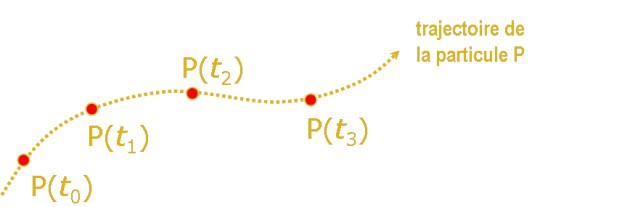
\includegraphics[scale=0.75]{trajectoire.jpg}
        \caption{Trajectoire}
    \end{minipage}\hfill
    \begin{minipage}[b]{0.4\linewidth}
         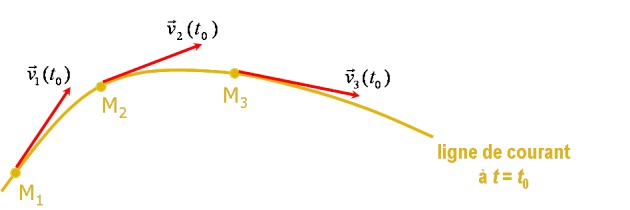
\includegraphics[scale=0.75]{courant.jpg}
        \caption{Ligne de courant}
    \end{minipage}
    \begin{minipage}[c]{0.4\linewidth}
       \begin{center}
 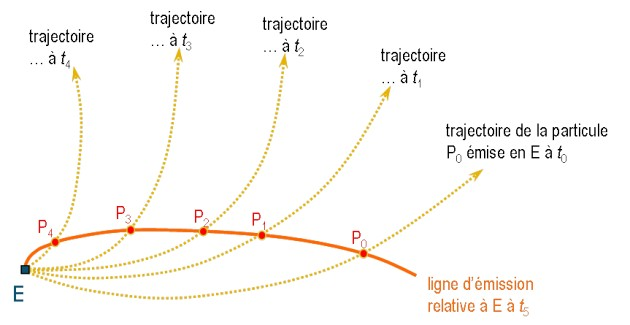
\includegraphics[scale=0.75]{emission.jpg}
\end{center}
        \caption{Ligne d'émission}
    \end{minipage}
\end{figure}
\paragraph{Remarque}Dans le cas d'un écoulement stationnaire (champ de vitesse indépendant du temps, statique), trajectoires, lignes de courant et lignes d'émission sont confondues.
\section{Analyse des déformations}
\subsection{Tenseur gradient de la transformation}
Soient le vecteur élémentaire infinitésimal $\dif\fv{X}$ de la configuration initiale et le vecteur élémentaire infinitésimal $\dif\fv{x}$ de la configuration déformée. On a $x_1=x_1(X_1, X_2, X_3)$, $x_2=...$ etc. d'où:
\begin{align*}
  \dif x_1&=\fpart{x_1}{X_1}\dif X_1+\fpart{x_1}{X_2}\dif X_2+\fpart{x_1}{X_3}\dif X_3\\
  \dif x_2&=\fpart{x_2}{X_1}\dif X_1+\fpart{x_2}{X_2}\dif X_2+\fpart{x_2}{X_3}\dif X_3\\
  \dif x_3&=\fpart{x_3}{X_1}\dif X_1+\fpart{x_3}{X_2}\dif X_2+\fpart{x_3}{X_3}\dif X_3\\
\end{align*}
que l'on peut réécrire sous forme matricielle: $\{\dif\fv{x}\}=[\fv{F}]\{\dif\fv{X}\}$ avec
$$[\fv{F}]=\left[\begin{array}{ccc}
    \fpart{x_1}{X_1}&\fpart{x_1}{X_2}&\fpart{x_1}{X_3}\\
    \fpart{x_2}{X_1}&\fpart{x_2}{X_2}&\fpart{x_2}{X_3}\\
    \fpart{x_3}{X_1}&\fpart{x_3}{X_2}&\fpart{x_3}{X_3}
\end{array}\right]$$
\fv{F} est le \emph{tenseur gradient de la transformation}:
$$\fv{F}=\left(\frac{\partial \fv{x}}{\partial \fv{X}}\right)^T\equiv (\nabla_0\fv{x})^T$$
où $\nabla_0$ est l'opérateur gradient par rapport à \fv{X}.
Le déterminant de \fv{F}, $J=\det \fv{F}$, est le \emph{jacobien} de la transformation.
\paragraph{}
\fv{F} est un tenseur régulier et possède donc un inverse $\fv{F}^{-1}$, car $\fv{F}\cdot \dif\fv{X}\neq 0$ pour $\dif\fv{X} \neq 0$.
\fv{F} peut être exprimé en fonction du vecteur déplacement:
$$\fv{F}=(\nabla_0 \fv{x})^T=(\nabla_0 (\fv{u}+\fv{X}))^T=(\nabla_0 \fv{u}+\fv{I})^T$$

\paragraph{}
Si $\fv{F}=\fv{I}$ en tout point du corps, alors celui-ci n'a pas tourné et n'a pas été déformé. Si \fv{F} est indépendant de \fv{X}, $\fv{F}(\fv{X},t)=\fv{F}(t)$, alors la déformation est dite \emph{homogène} (par exemple, les dilatations pures, les extensions simples, les cisaillements simples). L'application $\fv{x}=\fv{x}(\fv{X},t)$ est alors de la forme $$\fv{x}=\fv{A}\cdot\fv{X}+\fv{c}$$ où \fv{A} (tenseur) et \fv{c} (vecteur) sont constants (on a $\fv{F}=\fv{A}$). Ce dernier correspond à une translation uniforme du corps. Dans le cas d'une transformation \emph{hétérogène}, en revanche, il y a dépendance de \fv{F} par rapport à \fv{X} (par exemple, combinaison d'une extension et d'un cisaillement).
\subsection{Dilatation pure}
Si un cube matériel a des côtés de longueur $L$ et $l$ dans les configurations de référence et courante respectivement, alors la déformation est une \emph{dilatation pure} ou \emph{uniforme} et l'application de la déformation s'écrit:
$$\chi(\fv{X})=\lambda X_1\fv{ê}_1+\lambda X_2\fv{ê}_2+\lambda X_3\fv{ê}_3$$ où $\lambda=L/l$ et \fv{F} est représenté par la matrice
$$[\fv{F}]=\left[\begin{array}{ccc}
\lambda&0&0\\
0&\lambda&0\\
0&0&\lambda
\end{array}\right]$$ Si $\lambda=1$ la déformation est isochore.
\subsection{Extension simple}
Dans le cas d'une \emph{extension simple} dans la direction $X_1$, $$\chi(\fv{X})=(1+\alpha)X_1\fv{ê}_1+X_2\fv{ê}_2+X_3\fv{ê}_3$$ et $$[\fv{F}]=\left[\begin{array}{ccc}
1+\alpha&0&0\\
0&1&0\\
0&0&1
\end{array}\right]$$
\subsection{Cisaillement simple}
\label{cisaillement}
Un \emph{cisaillement simple} est une déformation telle qu'il existe un ensemble de lignes dont les longueurs et les orientations ne changent pas (carré $\longrightarrow$ parallélogramme par exemple).
$$\chi(\fv{X})=(X_1+\gamma X_2)\fv{ê}_1+X_2\fv{ê}_2+X_3\fv{ê}_3$$
et
$$[\fv{F}]=\left[\begin{array}{ccc}
1&\gamma&0\\
0&1&0\\
0&0&1
\end{array}\right]$$ $\gamma$ désigne la quantité de cisaillement.

\subsection{Tenseur des déformations de Green-Lagrange}
On s'intéresse ici à la variation des distances entre les points $P$ et $Q$ de la configuration initiale et les points $\bar{P}$ et $\bar{Q}$ de la configuration courante. On a:
$$(\dif s)^2-(\dif S)^2=\dif \fv{x}\cdot \dif \fv{x}-\dif \fv{X}\cdot \dif \fv{X}=\dif \fv{X}\cdot(\fv{F}^T\cdot\fv{F})\cdot \dif \fv{X}-\dif \fv{X}\cdot \dif \fv{X} \equiv 2\dif \fv{X}\cdot \fv{E} \cdot \dif \fv{X}$$
On a utilisé ici le \emph{tenseur des déformations de Green-Lagrange}:
$$\begin{aligned}
\fv{E}&=\frac{1}{2}(\fv{F}^T\cdot \fv{F}-\fv{I})\\
 &=\frac{1}{2}[\nabla_0\fv{u}+(\nabla_0\fv{u})^T + (\nabla_0\fv{u})\cdot(\nabla_0\fv{u})^T ]
 \end{aligned}
$$
Ce tenseur est symétrique. La variation de la distance est nulle, et donc le mouvement est rigide, ssi $\fv{E}=\fv{0}$.
Selon la notation indicielle, les composantes cartésiennes de \fv{E} s'écrivent:
$$E_{ij}=\frac{1}{2}\left(\frac{\partial u_j}{\partial X_i}+\frac{\partial u_i}{\partial X_j}+\frac{\partial u_k}{\partial X_i}\frac{\partial u_k}{\partial X_j}\right)$$
\paragraph{}
De manière générale, les vecteurs propres d'un tenseur de déformations sont appelées \emph{directions principales de déformation}, orthogonales aux \emph{plans principaux}, et les valeurs propres sont appelées \emph{déformations principales}.
\paragraph{}
Les composantes $E_{11}$, $E_{22}$ et $E_{33}$ sont les déformations normales (allongement relatif dans la direction $\fv{ê}_1$, $\fv{ê}_2$ ou $\fv{ê}_3$ resp.) tandis que les composantes $E_{12}$, $E_{23}$ et $E_{13}$ sont les déformations de cisaillement.
\paragraph{Dilatation pure:}
$$[E]=\frac{1}{2}
\left[\begin{array}{ccc}
\lambda^2-1&0&0\\
0&\lambda^2-1&0\\
0&0&\lambda^2-1\\
\end{array}\right]$$
\paragraph{Extension simple:}
$$[E]=\frac{1}{2}
\left[\begin{array}{ccc}
2\alpha+\alpha^2&0&0\\
0&0&0\\
0&0&0\\
\end{array}\right]$$
\paragraph{Cisaillement simple:}
$$[E]=\frac{1}{2}
\left[\begin{array}{ccc}
0&\gamma&0\\
\gamma&\gamma^2&0\\
0&0&0\\
\end{array}\right]$$

\subsection{Changement de volume et de surface}
Soit un volume infinitésimal $\dif V=\dif \fv{X}\cdot(\dif\fv{Y}\wedge \dif\fv{Z})=\det[\dif\fv{X}\dif\fv{Y}\dif\fv{Z}]$ d'un corps non déformé et le volume infinitésimal $\dif v=\det[\dif\fv{x}\dif\fv{y}\dif\fv{z}]$ obtenu après déformation. On a
$$\dif v=\det[[\fv{F}][\dif\fv{X}d\fv{Y}\dif\fv{Z}]]=\det[\fv{F}]\dif V$$
et donc $$\dif v=J\dif V.$$
\paragraph{}
Pour un élément infinitésimal de surface, on obtient: $$\dif\fv{a}=J\fv{F}^{-T}\dif\fv{A}.$$
\subsection{Tenseur des déformations infinitésimal}
\label{défo_infinit}
\paragraph{Hypothèses de petites perturbations (HPP):}
\begin{itemize}
\item $|\fv{u}|\ll 1\longrightarrow \mathcal{C}_0\approx \mathcal{C}_t$
\item $|\nabla_0\fv{u}|\ll 1\longrightarrow \nabla_0\approx\nabla,\,\,\fv{x}\approx\fv{X}$
\end{itemize}
\paragraph{}
Sous ces hypothèses, on peut négliger les termes non-linéaires du tenseur des déformations de Green-Lagrange. Le \emph{tenseur des déformations infinitésimal} est défini comme la partie linéaire de \fv{E}:
\begin{equation}
\label{eq:varespsilon}
\varepsilon=\frac{1}{2}[\nabla\fv{u}+(\nabla\fv{u})^T]
\end{equation}
\begin{equation}
\label{eq:varepsInd}
\varepsilon_{ij}=\frac{1}{2}\left(\frac{\partial u_j}{\partial x_i}+\frac{\partial u_i}{\partial x_j}\right)
\end{equation}
Les composantes de déformation diagonales sont les \emph{déformations normales infinitésimales}. Les autres composantes sont les \emph{déformations infinitésimales de cisaillement}. Les \emph{déformations de cisaillement conventionnelles} ou \emph{nominales} sont $\gamma_{12}=2\varepsilon_{12}$, $\gamma_{13}=2\varepsilon_{13}$ et $\gamma_{23}=2\varepsilon_{23}$ (voir section \ref{cisaillement}).
\paragraph{}
Dans le système de coordonnées cylindriques, le vecteur déplacement et l'opérateur $\nabla$ deviennent:
$$\fv{u}=u_r\fv{ê}_r+u_{\theta}\fv{ê}_{\theta}+u_z\fv{ê}_z$$
\begin{equation}\label{eq:nabla}\nabla=\fv{ê}_r\frac{\partial}{\partial r}+\frac{1}{r}\fv{ê}_{\theta}\frac{\partial}{\partial \theta}+\fv{ê}_z\frac{\partial}{\partial z}\end{equation}
$$\frac{\partial \fv{ê}_r}{\partial \theta}=\fv{ê}_{\theta},\qquad \frac{\partial \fv{ê}_{\theta}}{\partial \theta}=-\fv{ê}_{r} $$
Et donc, en injectant \eqref{eq:nabla} dans \eqref{eq:varespsilon} on obtient les composantes du tenseur des déformations infinitésimal dans le système de coordonnées cylindriques.

\section{\'Equations de compatibilité}
Le calcul de déformations (infinitésimales ou finies) à partir d'un champ de déplacement donné est un exercice direct. En revanche, le calcul des déplacements pour un champ de déformation donné n'est pas toujours possible. Il y a en effet 6 équations aux dérivées partielles indépendantes (reliant les déformations aux déplacements, voir relation \eqref{eq:varepsInd}) pour seulement trois déplacements inconnus, ce qui donne en général un système surdéterminé. Certaines conditions doivent être remplies pour assurer l'unicité du champ de déplacement.
\paragraph{}
Considérons les déformations infinitésimales d'un milieu bidimensionnel:
$$\begin{aligned}
\frac{\partial u_1}{\partial x_1}&=\varepsilon_{11},\\
\frac{\partial u_2}{\partial x_2}&=\varepsilon_{22},\\
\frac{\partial u_1}{\partial x_2}+\frac{\partial u_2}{\partial x_1}&=2\varepsilon_{12}
\end{aligned}$$
On obtient  la condition de compatibilité en dérivant deux fois la première équation par rapport à $x_2$, deux fois la deuxième équation par rapport à $x_1$ et la troisième équation une fois par rapport à chacune des variables $x_1$ et $x_2$:
$$\begin{aligned}
\frac{\partial^3 u_1}{\partial x_1\partial x_2^2}&=\frac{\partial^2\varepsilon_{11}}{\partial x_2^2},\\
\frac{\partial^3 u_2}{\partial x_2\partial x_1^2}&=\frac{\partial^2\varepsilon_{22}}{\partial x_1^2},\\
\frac{\partial^3 u_1}{\partial x_2^2\partial x_1}+\frac{\partial^3 u_2}{\partial x_1^2\partial x_2}&=2\frac{\partial^2\varepsilon_{12}}{\partial x_1\partial x_2}.
\end{aligned}$$
En injectant les deux premières équation dans la troisième, on obtient la \emph{condition de compatibilité des déformations} pour un problème d'élasticité en 2-D:
$$\frac{\partial^2\varepsilon_{11}}{\partial x_2^2}+\frac{\partial^2\varepsilon_{22}}{\partial x_1^2}=2\frac{\partial^2\varepsilon_{12}}{\partial x_1 \partial x_2}$$
\section{Tenseurs des taux de déformation et tourbillon}
\label{taux_defo_troub}
Le \emph{tenseur gradient de vitesse} $\fv{L}\equiv (\nabla \fv{v})^T$, utilisé plutôt en mécanique des fluides, détermine le taux de déformation. Il peut être exprimé comme la somme d'une partie symétrique et d'une partie antisymétrique:
$$\fv{L}=\frac{1}{2}[\nabla\fv{v}+(\nabla\fv{v})^T]-\frac{1}{2}[\nabla\fv{v}-(\nabla\fv{v})^T]\equiv \fv{D}+\mathbf{\Omega}$$
\paragraph{}
\fv{D} (symétrique) est le \emph{tenseur des taux de déformation} et $\mathbf{\Omega}$ (antisymétrique) est le \emph{tenseur des taux de rotations}.
\paragraph{}
Les composantes $D_{11}$, $D_{22}$ et $D_{33}$ sont les \emph{taux d'allongement ou de dilatation linéaire}. Les composantes $D_{12}$, $D_{13}$ et $D_{23}$ sont les \emph{taux de déformation de cisaillement}.
\paragraph{}
Puisque $\Omega_{11}=\Omega_{22}=\Omega_{33}=0$ et puisque $\mathbf{\Omega}$ est antisymétrique, il ne possède que trois composantes indépendantes:
$$\mathbf{\Omega}=\left[
\begin{array}{ccc}
0&-\omega_3&\omega_2\\
\omega_3&0&-\omega_1\\
-\omega_2&\omega_1&0
\end{array}\right]$$
Le \emph{vecteur rotation locale} ou \emph{vecteur tourbillon} est défini par
$$\mathbf{\omega}=\frac{1}{2}\text{rot}\fv{v}.$$
Un écoulement est irrotationnel si le vecteur tourbillon est nul.

\part{Vecteurs contrainte et tenseurs des contraintes}
\section{Vecteur contrainte, tenseur des contraintes et formule de Cauchy}

Une \emph{contrainte vraie} (ou \emph{contrainte de Cauchy}) est définie comme le quotient de la force et de la surface courante (déformée). Cette force ne dépend pas seulement de l'aire mais également de l'orientation de la surface, définie grâce à la normale à la surface\footnote{La direction de la normale est celle dans laquelle une vis avance lorsqu'elle tourne le long du contour de la surface.}. La surface est alors associée au vecteur $\fv{A}=A\fv{\^n}$. Une contrainte est donc un vecteur.
\paragraph{}
Soit $\Delta\fv{f}(\fv{\^n})$ la force agissant sur une petite surface $\Delta a$ localisée au point \fv{x}. Le vecteur contrainte est défini par: $$\fv{t}(\fv{\^n})=\lim_{\Delta a\rightarrow 0}\frac{\Delta\fv{f(\fv{\^n})}}{\Delta a}.$$ Le vecteur contrainte est en fait une fonction de (\fv{\^n}) et par le principe d'action-réaction on a $\fv{t}(-\fv{\^n})=-\fv{t}(\fv{\^n})$.
\paragraph{}
Essayons maintenant d'identifier les diverses composantes de la contrainte en un point $A$ \emph{interne} au milieu continu. Imaginons une boîte rectangulaire infinitésimale centrée en ce point dont les côtés sont parallèles aux axes des coordonnées. Pour un point $B$ situé en surface du milieu continu, cette boîte est un tétraèdre dont les 3 arrêtes orthogonales sont dans la direction des trois vecteurs de base du repère cartésien (voir Figure \ref{fig:tetra}).
\begin{figure}[!h]
 \centering
 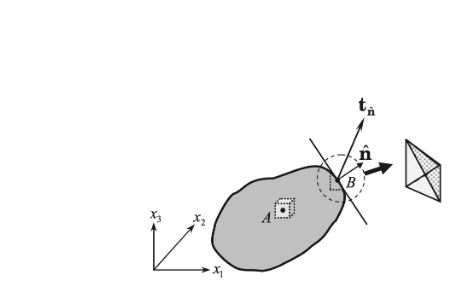
\includegraphics[scale=0.65]{./patate.jpg}
 \caption{Milieu continu et tétraèdre}
 \label{fig:tetra}
 \end{figure}
  Soient $-\fv{t}_1$, $-\fv{t}_2$, $-\fv{t}_3$ et $ \fv{t}$ les vecteurs contrainte dirigés vers l'extérieur sur les faces dont les normales sont $-\fv{ê}_1$,  $-\fv{ê}_2$, $-\fv{ê}_3$ et $\fv{\^n}$ respectivement. Par une habile somme des forces à la Newton\footnote{Voir page 110 du livre de Reddy pour le développement.}, on obtient $$\fv{t}=\fv{\^n}\cdot(\fv{ê}_1\fv{t}_1+\fv{ê}_2\fv{t}_2+\fv{ê}_3\fv{t}_3).$$
On pose $\boldsymbol{\sigma}\equiv\fv{ê}_1\fv{t}_1+\fv{ê}_2\fv{t}_2+\fv{ê}_3\fv{t}_3$. $\boldsymbol{\sigma}$ est appelé le \emph{tenseur des contraintes}. La \emph{formule des contraintes de Cauchy} permet de relier le tenseur des contraintes au vecteur contrainte en un point de la frontière du milieu continu:
$$\fv{t}=\fv{\^n}\cdot\boldsymbol{\sigma}=\boldsymbol{\sigma}^T\cdot\fv{\^n}.$$
Ce tenseur est symétrique et donc diagonalisable. Sous forme matricielle:
$$\left\{\begin{array}{c}
t_1\\
t_2\\
t_3
\end{array}\right\}
=\left[
\begin{array}{ccc}
\sigma_{11}&\sigma_{21}&\sigma_{31}\\
\sigma_{12}&\sigma_{22}&\sigma_{32}\\
\sigma_{13}&\sigma_{23}&\sigma_{33}\\
\end{array} \right]
\left\{\begin{array}{c}
n_1\\
n_2\\
n_3
\end{array}\right\}$$
\paragraph{}
La composante $\sigma_{ij}$ représente la contrainte (densité de force de contact) agissant sur un plan (``facette'') perpendiculaire à la direction $\fv{ê}_j$ et dans la direction $\fv{ê}_i$. Donc, si l'on considère maintenant un parallélépipède dont les faces sont orthogonales aux vecteurs d'une base orthonormée ($\fv{ê}_i$), les 3 composantes du vecteur contrainte sur la facette de normale $\fv{ê}_i$ sont les composantes $\sigma_{i1}$, $\sigma_{i2}$ et $\sigma_{i3}$ du tenseur des contraintes dans cette base.
\paragraph{}
La \emph{contrainte normale} est la composante de \fv{t} dans la direction de \fv{\^n} et s'obtient donc simplement par
\begin{equation}
\label{eq:tnn}
t_{nn}=\fv{t}\cdot\fv{\^n}=n_j\sigma_{ji}n_i.
\end{equation}
\paragraph{}
La \emph{contrainte de cisaillement} est la composante perpendiculaire à la direction de \fv{\^n}. Par Pythagore:
\begin{equation}
\label{eq:tau}
t_{ns}\equiv\tau=\sqrt{|\fv{t}|^2-t_{nn}^2}.
\end{equation}
\paragraph{}
Les composantes d'un tenseur des contraintes $\boldsymbol{\sigma}$ dans une base cartésienne peuvent être exprimées en fonction de ses composantes dans une autre base elle aussi cartésienne: $$[\boldsymbol{\sigma}']=\fv{L}[\boldsymbol{\sigma}]\fv{L}^T$$.
\section{Contraintes principales}
On s'intéresse ici à la détermination des valeurs maximales des contraintes normales et de cisaillement en un point fixé pour un état de contrainte donné. Le but est de pouvoir détecter si les valeurs maximales admissibles (de contrainte normale ou de cisaillement), appelées résistances, sont dépassées.
\paragraph{}
Les valeurs maximales portent le nom de \emph{valeurs principales} et sont notées $\sigma_i$. Ce sont les valeurs propres du tenseur des contraintes. Les plans sur lesquelles elles se produisent sont les \emph{plans principaux}, caractérisés par les vecteurs propres associés $\fv{\^n}_i$ (les \emph{directions principales des contraintes}). On a $\boldsymbol{\sigma}=\sum_{i=1}^3 \sigma_i\,\fv{\^n}_i\fv{\^n}_i$. Par convention on rangera les contraintes principales par ordre décroissant: $\sigma_1\geq \sigma_2\geq\sigma_3$ avec $\sigma_1$ la contrainte normale maximale et $\sigma_3$ la minimale.
\paragraph{}
La base orthonormée $(\fv{\^n}_1,\fv{\^n}_2,\fv{\^n}_3)$ est la base principale, et la matrice du tenseur des contraintes de Cauchy dans cette base est diagonale:
$$[\sigma]_{principal}=\left[
\begin{array}{ccc}
\sigma_1&0&0\\
0&\sigma_2&0\\
0&0&\sigma_3
\end{array}\right]$$

\section{Représentation de Mohr}
La représentation de Mohr permet de visualiser comment varie le vecteur contrainte en un point matériel quand on change l'orientation de la facette.
Soient $(n_1, n_2, n_3)$ les coordonnées d'un vecteur dans la base formée par les vecteurs principaux $(\fv{\^n}_1,\fv{\^n}_2,\fv{\^n}_3)$ de $\boldsymbol{\sigma}$ données et fixées.
Par \ref{eq:tnn} on a:
$$t_{nn}=\sigma_1n_1^2+\sigma_2n_2^2+\sigma_3n_3^2$$
et par \ref{eq:tau} on a:
$$\tau^2+t_{nn}^2=\sigma_1^2 n_1^2+\sigma_2^2 n_2^2+\sigma_3^2 n_3^2.$$ En rajoutant une équation pour fixer la norme de \fv{\^n} à 1, on obtient 3 équations qui nous permettent d'isoler $n_1^2$, $n_2^2$ et $n_3^2$. La contrainte de positivité sur ces derniers nous amène finalement aux trois inéquations suivantes, représentant des cercles dans le plan de Mohr ($t_{nn},\tau$) (les \emph{cercles de Mohr}):
$$\begin{aligned}
  \left(t_{nn}-\frac{\sigma_2+\sigma_3}{2}\right)^2+\tau^2&\geq \left(\frac{\sigma_2-\sigma_3}{2}\right)^2\\
  \left(t_{nn}-\frac{\sigma_3+\sigma_1}{2}\right)^2+\tau^2&\leq \left(\frac{\sigma_3-\sigma_1}{2}\right)^2\\
  \left(t_{nn}-\frac{\sigma_1+\sigma_2}{2}\right)^2+\tau^2&\geq \left(\frac{\sigma_1-\sigma_2}{2}\right)^2\\
\end{aligned}$$
Les termes de droite représentent les rayons des cercles au carré, tandis que les centres sont $\left(\frac{\sigma_1+\sigma_2}{2},0\right)$, $\left(\frac{\sigma_1+\sigma_3}{2},0\right)$ et $\left(\frac{\sigma_2+\sigma_3}{2},0\right)$.
\paragraph{}
Ces inégalités signifient que l'extrémité du vecteur contrainte \fv{t} de coordonnée ($t_{nn},\tau$) dans le plan de Mohr se situe à l'extérieur des 2 petits cercles et à l'intérieur du grand (voir zone bleue de la Figure \ref{fig:mohr}).
\begin{figure}[!h]
\centering
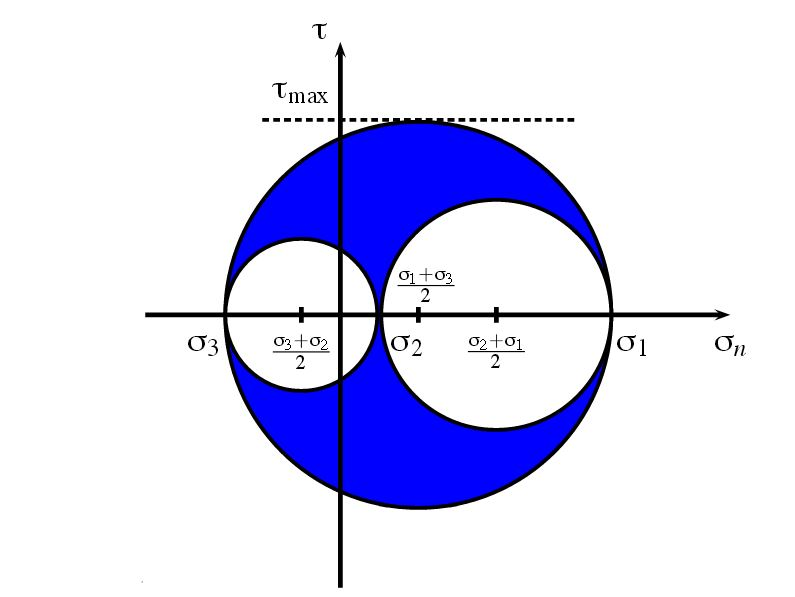
\includegraphics[width = 0.8\textwidth]{./mohr}
\caption{Les trois cercles de Mohr}
\label{fig:mohr}
\end{figure}
Réciproquement, tout point $(t_{nn},\tau)$ de la zone bleue est atteint pour une direction \fv{\^n}. En particulier, les frontières du domaine formées par les cercles sont atteintes respectivement pour $n_3=0$, $n_1=0$ et $n_2=0$.
\paragraph{Théorème du cisaillement maximal:} Soit $\boldsymbol{\sigma}$ le tenseur des contraintes en un point
matériel; la contrainte tangentielle $\tau_{max}$ maximale subie sur les facettes lorsqu'on fait varier
les normales \fv{\^n} vaut $\frac{\sigma_1-\sigma_3}{2}$ et s'exerce sur les facettes contenant la direction $\fv{\^n}_2$, à  $\pm \pi/4$ des directions $\fv{\^n}_1$ et $\fv{\^n}_3$.
\paragraph{}
Ce résultat est visible sur la Figure \ref{fig:mohr}.

\section{\'Etats de contraintes remarquables}
Les Figures \ref{fig:ts}, \ref{fig:cs} et \ref{fig:ba} donnent un récapitulatif des états de contraintes remarquables.

\begin{figure}[!h]
\centering
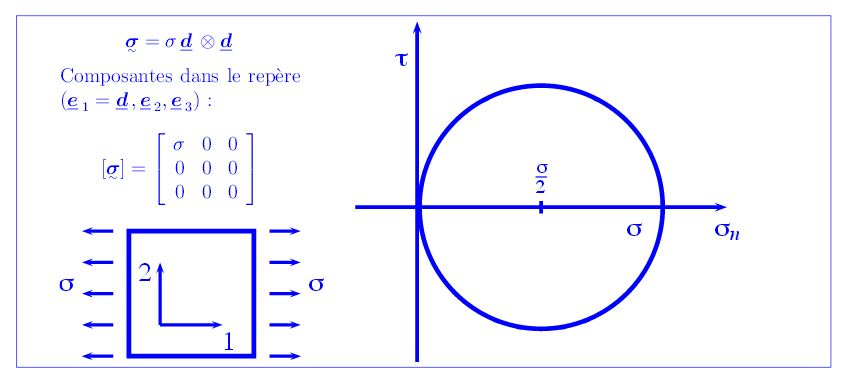
\includegraphics[scale=0.6]{./tractionsimple}
\caption{Récapitulatif: état de traction simple}
\label{fig:ts}
\end{figure}

\begin{figure}[!h]
\centering
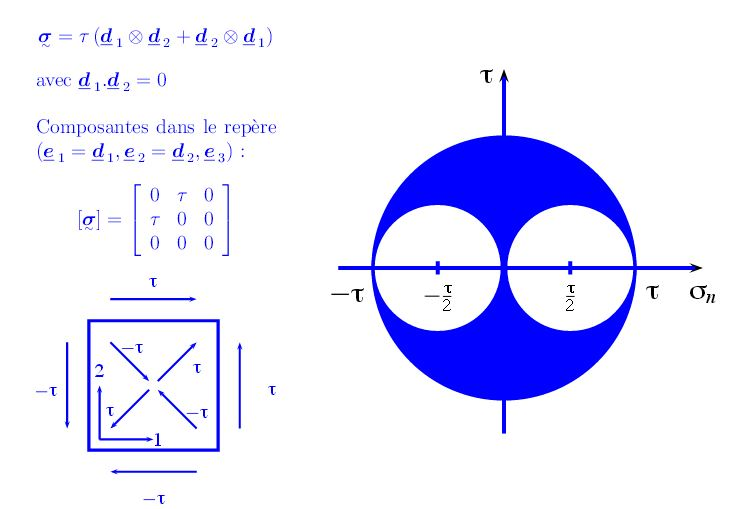
\includegraphics[scale=0.6]{./cisaillementsimple}
\caption{Récapitulatif: cisaillement simple}
\label{fig:cs}
\end{figure}

\begin{figure}[!h]
\centering
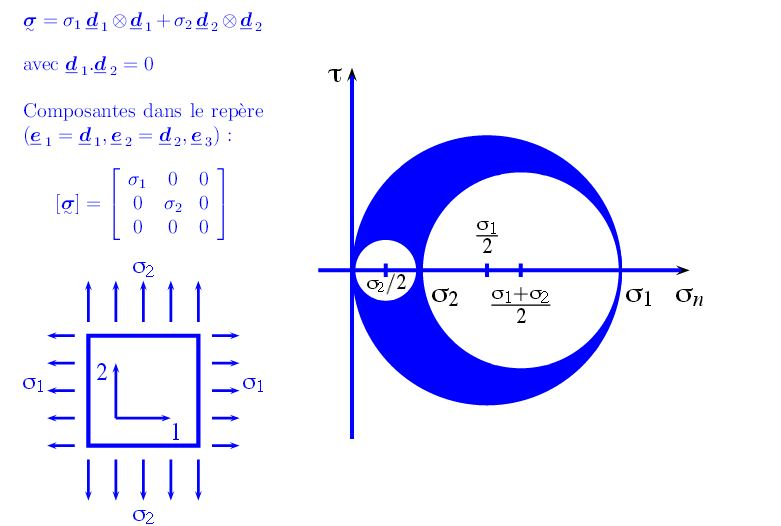
\includegraphics[scale=0.6]{./biaxial}
\caption{Récapitulatif: état de contrainte bi-axial}
\label{fig:ba}
\end{figure}

\part{Lois de conservation}
\section{Théorème du transport de Reynolds}
On veut pouvoir étudier la conservation de la masse sur un volume matériel
$\Omega (t)=\{\fv{x}(\fv{X},t)|\fv{X}\in \Omega_0\}$,
à savoir
$$\fdif{}{t}\mathcal{M}(t)=\fdif{}{t}\int_{\Omega (t)}\rho(\fv{x},t) \dif v=0.$$
Il nous faut donc calculer une intégrale sur un volume en déformation!
C'est ce que va nous permettre de faire le théorème du transport de Reynolds (TTR).

Soit $\mathcal{I}(t)=\int_{\Omega (t)}\phi(\fv{x},t) \dif v$.
Pour appliquer la dérivée temporelle matérielle $\frac{D}{Dt}\mathcal{I}(t)$,
on retourne à la configuration de référence et aux coordonnées matérielles:
$$\mathcal{I}(t)=\int_{\Omega_0}\phi(\fv{X},t) J \dif V$$
avec $J=\det(\fv{F})$ le jacobien de la transformation.
Le domaine d'intégration ne varie donc plus et on peut appliquer la dérivée à l'intégrant:
$$\frac{D}{Dt}\mathcal{I}(t)=\int_{\Omega_0}\left(\fpart{\phi(\fv{X},t)}{t}J
+\phi(\fv{X},t)\fpart{J}{t}\right) \dif V$$
La formule d'Euler nous donnant: $\frac{\partial J}{\partial t}=J\nabla\cdot\fv{v}$ on obtient:
$$\begin{aligned}
\frac{D}{Dt}\mathcal{I}(t)&=\int_{\Omega_0}\left(\frac{\partial \phi(\fv{X},t)}{\partial t}+\phi(\fv{X},t)\nabla\cdot\fv{v}\right)JdV\\
 &=\int_{\Omega_0}\left(\frac{D}{Dt}\phi(\fv{X},t)+\phi(\fv{X},t)\nabla\cdot\fv{v}\right)JdV \qquad\text{(Par définition de } \frac{D}{Dt}\text{ en description lagrangienne)}\\
 &=\int_{\Omega (t)}\left(\frac{D}{Dt}\phi(\fv{x},t)+\phi(\fv{x},t)\nabla\cdot\fv{v}\right) \dif v\qquad\text{(Retour aux coordonnées eulériennes) }\\
 &=\int_{\Omega (t)}\left(\frac{\partial\phi}{\partial t}+\fv{v}\cdot\nabla\phi+\phi\nabla\cdot\fv{v}\right) \dif v\qquad\text{(Par définition de } \frac{D}{Dt}\text{ en description eulérienne)}\\
 &=\int_{\Omega (t)}\left(\frac{\partial\phi}{\partial t}+\nabla\cdot(\phi\fv{v})\right) \dif v
\end{aligned}$$
En appliquant le théorème de la divergence, on obtient le TTR:
$$\boxed{
\begin{aligned}
\frac{D}{Dt}\mathcal{I}(t) &=\int_{\Omega (t)}\left(\frac{D}{Dt}\phi+\phi\nabla\cdot\fv{v}\right) \dif v\qquad\\
 & =\int_{\Omega (t)}\left(\frac{\partial \phi}{\partial t}+\nabla\cdot(\phi\fv{v})\right) \dif v\\
 & = \int_{\Omega (t)}\frac{\partial\phi}{\partial t} \dif v+\oint_{\partial \Omega (t)}\phi\fv{v}\cdot\fv{\^n} \dif s\\
\end{aligned}}$$
La première expression est plus ``lagrangienne'' (variation en suivant le point matériel + déformation du volume associé à ce volume matériel), tandis que la deuxième expression est plutôt ``eulérienne'' (variation en un point fixé + flux à travers la surface).
\paragraph{Remarque} La formule de Leibniz en 1 dimension est un cas particulier du TTR:
\[ \fdif{}{t}\int_{a(t)}^{b(t)}f(x,t) \dif x =
\int_{a(t)}^{b(t)}\fpart{f}{t} \dif x + f(b(t),t)\fdif{b}{t} - f(a(t),t)\fdif{a}{t}. \]

Ce théorème exprime la variation temporelle d'une intégrale sur une région matérielle $\Omega$, région dont la frontière $\partial \Omega$ se déplace avec la vitesse du fluide $\fv{v}(\fv{x},t)$ ($\Omega$ se déforme donc à une vitesse \fv{v}). Cette région contient donc une masse fixe car aucune masse ne traverse sa frontière.

Si par contre, on choisit une région $\Omega$ dont chaque point à la surface se déplace à vitesse $\fv{v}_s$, on obtient la dérivée temporelle ``arbitraire'':
\begin{equation}
  \fdif{}{t}\int_{\Omega (t)}\phi(\fv{x},t) \dif v=\int_{\Omega (t)}\fpart{\phi}{t} \dif v + \oint_{\partial \Omega (t)}\phi\fv{v}_s\cdot \fv{\^n} \dif s
\end{equation}

La région $\Omega$, appelée \emph{volume de contrôle}, ne se déforme plus suivant le milieu (voir Fig \ref{fig:volmat} et Fig \ref{fig:volcont}).

\begin{figure}
    \begin{minipage}[b]{0.4\linewidth}
        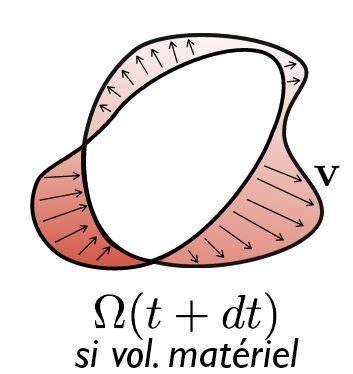
\includegraphics[scale=0.5]{volmateriel.jpg}
        \caption{Volume matériel}
        \label{fig:volmat}
    \end{minipage}\hfill
    \begin{minipage}[b]{0.4\linewidth}
         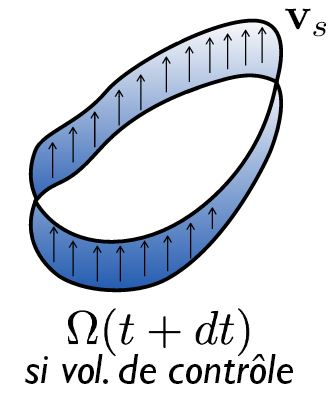
\includegraphics[scale=0.5]{volcontrole.jpg}
         \caption{Volume de contrôle}
         \label{fig:volcont}
    \end{minipage}
\end{figure}

On peut maintenant faire le lien entre la dérivée de l'intégrale sur un volume de contrôle et sur un volume matériel:
\begin{equation}
  \label{comparaison_mat_cont}
  \boxed{\fdif{}{t}\int_{\Omega (t)}\phi(\fv{x},t) \dif v = \frac{D}{Dt}\int_{\Omega (t)}\phi(\fv{x},t) \dif v + \oint_{\partial \Omega (t)}\phi(\fv{x},t)(\fv{v}_s-\fv{v})\cdot \fv{\^n} \dif s}
\end{equation}
Le dernier terme à droite représente le flux total pour la grandeur $\phi$ qui sort du volume de contrôle $\Omega$.

\section{Conservation de la masse en description eulérienne}
Le principe de conservation de la masse indique de manière générale que la masse totale de toute partie d'un corps reste constante indépendamment de son mouvement:
\[ \frac{D}{Dt}\mathcal{M}(t)=\frac{D}{Dt}\int_{\Omega (t)}\rho \dif v = 0 \]
On applique donc TTR avec $\phi=\rho$:
\[ \int_{\Omega (t)}\left(\frac{D\rho}{Dt} + \rho\nabla\cdot\fv{v}\right) \dif v =
\int_{\Omega (t)}\left(\fpart{\rho}{t} + \nabla\cdot(\rho\fv{v})\right) \dif v = 0 \]
L'intégrale s'annulant pour toute région $\Omega$, l'intégrant doit être nul.
Cela nous donne la forme locale de la conservation de la masse (\emph{équation de continuité}):
\[ \boxed{
    \begin{aligned}
      \frac{D\rho}{Dt}+\rho\nabla\cdot\fv{v} & = 0 \\
      \frac{\partial \rho}{\partial t}+\nabla\cdot(\rho\fv{v}) & = 0.
    \end{aligned}
} \]

Dans le cas d'un écoulement stationnaire ($\fpart{(\cdot)}{t} = 0$),
l'équation de continuité se résume à
\[ \nabla\cdot(\rho\fv{v}) = 0. \]

Si le milieu est incompressible ou multiphasique immiscible incompressible ($\frac{D\rho}{Dt}=0$),
on a
\[ \nabla\cdot\fv{v} = 0 \]

Prenons maintenant l'équation~\eqref{comparaison_mat_cont}.
Pour un volume de contrôle immobile, $\fv{v}_s = 0$, on a donc
\[ \frac{D}{Dt}\int_{\Omega (t)}\rho \dif v = \fdif{}{t}\int_{\Omega (t)}\rho  \dif v+\oint_{\partial\Omega (t)}\rho\fv{v}\cdot\fv{\^n} \dif s=0. \]
En effet, la dérivée temporelle de la masse du système est égale à la dérivée temporelle de la masse du volume de contrôle à laquelle on ajoute le débit massique à travers la surface de contrôle
\footnote{Le tout étant nul par conservation de la masse.}.
On obtient donc l'équation de conservation de la masse dans un volume de contrôle fixe:
\[ \fdif{}{t}\int_{\Omega }\rho \dif v = -\oint_{\partial\Omega} \rho\fv{v}\cdot\fv{\^n} \dif s \]
Pour un écoulement stationnaire cela donne
\[ 0 = -\oint_{\partial\Omega}\rho\fv{v}\cdot\fv{\^n} \dif s = \rho_1v_1A_1-\rho_2v_2A_2. \]

\section{Variante du théorème de transport de Reynolds}
En considérant un \emph{débit massique} $\phi = \rho Q$ avec $Q = Av$ le débit volumique, le TTR nous fournit:
\begin{align*}
  \frac{D}{Dt}\int_{\Omega (t)}\rho Q(\fv{x},t) \dif v & = \int_{\Omega (t)}\frac{D(\rho Q)}{Dt} + \rho Q \div{\fv{v}} \dif v\\
                                                       & = \int_{\Omega (t)}\rho\frac{DQ}{Dt} + Q\left(\frac{D\rho}{Dt} + \rho\div{\fv{v}}\right) \dif v
\end{align*}
ce qui donne, par la conservation de la masse, la variante du théorème de Reynolds:
\begin{equation}
  \label{ttr2}
  \boxed{\frac{D}{Dt}\int_{\Omega (t)}\rho Q \dif v=\int_{\Omega(t)}\rho\frac{DQ}{Dt} \dif v.}
\end{equation}

\section{Conservation de la quantité de mouvement et du moment cinétique}
Le principe de conservation de la quantité de mouvement $\fv{P}=m\fv{v}$, ou seconde loi de Newton, stipule : $$\fdif{}{t}\fv{P}=\fdif{}{t}m\fv{v}=\fv{F}$$ avec \fv{F} la résultante des forces extérieures. Pour une masse constante, on retrouve $\fv{F}=m\fv{a}$.
\paragraph{}
Dans le cas d'un milieu continu, on a: $$\fv{P}(t)=\int_{\Omega(t)}\rho\fv{v} \dif v.$$
Les forces agissant sur le volume peuvent être des forces volumiques agissant à distance sur la distribution de masse (gravité,...)
\footnote{\fv{f} est exprimé en $\newton\cdot\kilogram^{-1}$ et \fv{t} (vecteur contrainte de surface) en $\newton\cdot\meter^{-2}$}: $$\fv{F}^d=\int_{\Omega (t)}\rho\fv{f} \dif v$$  ou des forces de contact (surfaciques): $$\fv{F}^c=\int_{\partial \Omega (t)}\fv{t} \dif s=\int_{\partial \Omega (t)}\fv{\^n}\cdot\boldsymbol{\sigma} \dif s.$$ Ces forces sont appelées forces \emph{extérieures}, et induisent des forces \emph{intérieures} qui résistent à la tendance d'un partie du milieu continu à être séparé du reste.
\paragraph{}
La conservation de la quantité du mouvement implique :
$$\frac{D}{Dt}\int_{\Omega (t)}\rho\fv{v} \dif v=\int_{\Omega (t)}\rho\fv{f} \dif v+\int_{\partial\Omega (t)}\fv{\^n}\cdot\boldsymbol{\sigma} \dif s$$
En appliquant la variante du théorème du transport de Reynolds (équation~\eqref{ttr2}) et le théorème de la divergence de Green-Ostrogradski, on arrive à la forme globale de l'équation du mouvement:
$$\int_{\Omega (t)}\left(\rho\frac{D\fv{v}}{Dt}-\rho\fv{f}-\nabla\cdot\boldsymbol{\sigma}\right) \dif v=0$$
On obtient alors la forme locale de la conservation de la quantité de mouvement:
$$\boxed{\rho\frac{D\fv{v}}{Dt}=\rho\fv{f}+\nabla\cdot\boldsymbol{\sigma}}$$
avec $\frac{D\fv{v}}{Dt}=\frac{\partial \fv{v}}{\partial t}+\fv{v}\cdot\nabla\fv{v}=\fv{a}$. En notation indicielle dans un repère cartésien cela donne:
$$\rho\left(\frac{\partial v_i}{\partial t}+v_j\frac{\partial v_i}{\partial x_j}\right)=\rho f_i+\frac{\partial \sigma_{ji}}{\partial x_j}.$$
\paragraph{}
Pour un état stationnaire, $\frac{\partial\fv{v}}{\partial t}=0$, d'où $$\nabla\cdot\boldsymbol{\sigma}+\rho\fv{f}=\rho\fv{v}\cdot\nabla\fv{v}$$
Si en plus les déformations sont infinitésimales (ex: solide en équilibre statique)\footnote{Cette relation peut s'obtenir en faisant un bilan de forces sur un volume élémentaire.}, $\fv{v}\cdot\nabla\fv{v}=0$ et
$$\nabla\cdot\boldsymbol{\sigma}+\rho\fv{f}=0.$$
\paragraph{}
Repartons maintenant de la forme de départ et essayons de déterminer la conservation de la quantité de mouvement dans un volume de contrôle fixe\footnote{Application: voir slides cours 6 (turbofan).}:
$$\frac{D}{Dt}\int_{\Omega(t)}\rho\fv{v} \dif v=\fv{F}$$
Par l'équation~\eqref{comparaison_mat_cont}, avec $\phi=\rho\fv{v}$ et sachant que $\fv{v}_s=0$, on aboutit à:
$$\fdif{}{t}\int_{\Omega }\rho\fv{v}\,  \dif v=\frac{D}{Dt}\int_{\Omega}\rho\fv{v} \dif v-\oint_{\partial\Omega }\rho\fv{v}\fv{v}\cdot\fv{\^n} \dif s$$
$$\Leftrightarrow$$
$$\fv{F}=\fdif{}{t}\int_{\Omega}\rho\fv{v}\,  \dif v+\oint_{\partial\Omega }\rho\fv{v}\fv{v}\cdot\fv{\^n} \dif s$$

\section{Conservation du moment de la quantité de mouvement}
Le moment d'une quantité $\omega(\fv{x},t)$ est définie par $$\fv{L}=\fv{x}\wedge\omega(\fv{x},t).$$
Le principe de conservation du moment cinétique indique que la variation temporelle du moment cinétique total \fv{L} d'un milieu continu est égal à la somme vectorielle des moments des forces extérieures qui agissent sur le milieu:
$$\frac{D\fv{L}}{Dt}=\frac{D}{Dt}\int_{\Omega (t)}\rho\fv{x}\wedge\fv{v} \dif v=\fv{M}^d+\fv{M}^c.$$
$\fv{M}^d$ est le moment des forces volumiques agissant à distance, $$\fv{M}^d=\int_{\Omega (t)}\fv{x}\wedge\rho\fv{f} \dif v$$ et $\fv{M}^c$ est le moment des forces de contact,
$$\fv{M}^c=\int_{\partial\Omega (t)}\fv{x}\wedge\fv{t} \dif s.$$
L'application de l'équation~\eqref{comparaison_mat_cont} conduit à :
$$\fdif{}{t}\int_{\Omega (t)}\rho\fv{x}\wedge\fv{v} \dif v=\frac{D}{Dt}\int_{\Omega (t)}\rho\fv{x}\wedge\fv{v} \dif v+\oint_{\partial\Omega (t)}\rho\fv{x}\wedge\fv{v}(\fv{v}_s-\fv{v})\cdot\fv{\^n} \dif s$$
On trouve alors la conservation du moment cinétique pour un volume de contrôle fixe\footnote{Application: voir slides cours 6.}
$$\fv{M}=\fdif{}{t}\int_{\Omega}\fv{x}\wedge\rho\fv{v} \dif v+\oint_{\partial\Omega }(\fv{x}\wedge\rho\fv{v})\fv{v}\cdot\fv{\^n} \dif s$$
\paragraph{}
On recherche maintenant la forme locale de la loi de conservation. Par TTR (variante), on a
$$\begin{aligned}
\frac{D}{Dt}\int_{\Omega (t)}\rho\fv{x}\wedge\fv{v} \dif v &=\int_{\Omega (t)}\rho\frac{D}{Dt}(\fv{x}\wedge\fv{v}) \dif v\\
 &=\int_{\Omega (t)}\rho \left(\frac{D\fv{x}}{Dt}\wedge\fv{v}+\fv{x}\wedge\frac{D\fv{v}}{Dt}\right) \dif v\\
  & =\fv{M}^c+\fv{M}^d\\
\end{aligned}$$
On va supposer que les forces de volume \fv{f} n'induisent pas de couple volumiques (le milieu est supposé non-polaire), donc $\frac{D\fv{x}}{Dt}\wedge\fv{v}=0$:
$$\int_{\Omega (t)}\underbrace{\rho \left(\fv{x}\wedge\frac{D\fv{v}}{Dt}\right)}_{e_{ijk}\rho x_j\frac{Dv_k}{Dt}} \dif v=\fv{M}^c+\fv{M}^d.$$
Exprimons $\fv{M}^c$ et $\fv{M}^d$ en notation indicielle:
$$\begin{aligned}
M_i^c&=\int_{\partial\Omega (t)}e_{ijk}x_jt_kds\\
 & =\int_{\partial\Omega (t)}e_{ijk}x_jn_l\sigma_{lk}ds & \text{  (car } t_k=n_1\sigma_{1k}+n_2\sigma_{2k}+n_3\sigma_{3k}\text{)}\\
 &=\int_{\Omega (t)}\frac{\partial}{\partial x_l}(e_{ijk}x_j\sigma_{lk}) \dif v& \text{(théorème de la divergence)}\\
 &=\int_{\Omega (t)}e_{ijk}\left(\frac{\partial x_j}{\partial x_l}\sigma_{lk}+x_j\frac{\partial\sigma_{lk}}{\partial x_l}\right) \dif v\\
 M_i^d&=\int_{\Omega (t)}e_{ijk}x_j\rho f_k \dif v
\end{aligned}$$
On a donc comme équations:
$$\int_{\Omega (t)}e_{ijk}\rho x_j\frac{Dv_k}{Dt} \dif v=\int_{\Omega (t)}e_{ijk}\left(\frac{\partial x_j}{\partial x_l}\sigma_{lk}+x_j\frac{\partial\sigma_{lk}}{\partial x_l}\right) \dif v+\int_{\Omega (t)}e_{ijk}x_j\rho f_k \dif v$$
ou encore:
$$\int_{\Omega (t)}e_{ijk}x_j\left(\rho\frac{Dv_k}{Dt}-\rho f_k-\frac{\partial \sigma_{lk}}{\partial x_l}\right) \dif v - \int_{\Omega (t)}e_{ijk}\underbrace{\frac{\partial x_j}{\partial x_l}}_{\delta_{jl}}\sigma_{lk} \dif v=0$$
Par conservation de la quantité de mouvement, le terme entre parenthèses est nul. La forme locale se résume donc à $e_{ijk}\sigma_{jk}=0$. En d'autres mots, le tenseur des contraintes doit être symétrique:
$$\boxed{\boldsymbol{\sigma}=\boldsymbol{\sigma}^T}$$

\section{Conservation de l'énergie et premier principe de la thermodynamique}
\subsection{Théorème de l'énergie cinétique}
On part de l'équation de conservation de la quantité du mouvement, multipliée scalairement par le champ de vitesses:
$$\rho\frac{D\fv{v}}{Dt}\cdot\fv{v}=\rho\fv{f}\cdot\fv{v}+(\nabla\cdot\boldsymbol{\sigma})\cdot\fv{v}$$
De plus, $$\frac{D\fv{v}}{Dt}\cdot\fv{v}=\frac{1}{2}\frac{D}{Dt}(\fv{v}\cdot\fv{v})\qquad\text{(énergie cinétique massique)}$$
En intégrant sur un volume matériel:
$$\int_{\Omega (t)}\frac{1}{2}\rho\frac{D}{Dt}(\fv{v}\cdot\fv{v}) \dif v=\int_{\Omega (t)}(\rho\fv{f}\cdot\fv{v}+(\nabla\cdot\boldsymbol{\sigma})\cdot\fv{v}) \dif v$$
On a:
\begin{align*}
(\nabla\cdot\boldsymbol{\sigma})\cdot\fv{v}&=\frac{\partial \sigma_{ji}}{\partial x_j}v_i=\frac{\partial}{\partial x_j}(\sigma_{ji}v_i)-\sigma_{ji}\frac{\partial v_i}{\partial x_j}\\
 &=\nabla\cdot(\boldsymbol{\sigma}^T\cdot\fv{v})-\boldsymbol{\sigma}:(\nabla\fv{v})^T\\
\end{align*}
Par le théorème de la divergence et par associativité du produit scalaire,
\begin{align*}
  \int_{\Omega (t)}\nabla\cdot(\boldsymbol{\sigma}\cdot\fv{v}) \dif v
  & = \oint_{\partial \Omega (t)}(\sp{\fv{\^n}}{\boldsymbol{\sigma}}) \cdot \fv{v} \dif s\\
  & = \oint_{\partial \Omega (t)}\fv{t}\cdot\fv{v} \dif s.
\end{align*}
On utilise ensuite la symétrie de $\boldsymbol{\sigma}$ et le fait que $(\nabla\fv{v})^T=\boldsymbol{\Omega}+\fv{D}$ (voir section \ref{taux_defo_troub}) et la propriété $\fv{A}^{sym}:\fv{B}^{antisym}=0$ pour déduire que $\boldsymbol{\sigma}:(\nabla\fv{v})^T=\boldsymbol{\sigma}:\fv{D}$. Cela nous mène enfin au \emph{théorème de l'énergie}:

$$\boxed{\frac{D}{Dt}\int_{\Omega (t)}\rho\frac{\fv{v}\cdot\fv{v}}{2} \dif v=\int_{\Omega (t)}\rho\fv{f}\cdot\fv{v} \dif v+\oint_{\partial \Omega (t)}\fv{t}\cdot\fv{v} \dif s-\int_{\Omega (t)}\boldsymbol{\sigma}:\fv{D} \dif v}$$

$$\frac{D}{Dt}K=\underbrace{W^d}_{\text{puissances des forces volumiques}}+\underbrace{W^c}_{\text{puissances des forces de contact}}-\underbrace{W^i}_{\text{puissances des efforts internes}}$$
Le terme $\boldsymbol{\sigma}:\fv{D}$ est nommé \emph{puissance de contrainte}.
\subsection{Conservation de l'énergie interne}
Le premier principe de la thermodynamique peut être résumé par l'équation \begin{equation}\label{eq:premier_principe}\frac{D}{Dt}(K+U)=W+H,\end{equation} $K$ étant l'énergie cinétique associée aux mouvements macroscopiques du milieu continu, $U$ l'énergie interne, $W$ la \fv{puissance} fournie et $H$ le taux de chaleur reçue par le système. Pour obtenir la forme globale de l'équation de l'énergie, détaillons chacun de ces termes.
\paragraph{}
L'énergie cinétique est donnée par $$K=\frac{1}{2}\int_{\Omega (t)}\rho\fv{v}\cdot\fv{v} \dif v$$ avec \fv{v} le vecteur vitesse.
\paragraph{}
L'énergie interne est quant à elle donnée par $$U=\int_{\Omega (t)}\rho e \dif v$$ où $e$ est l'énergie interne par unité de masse. L'énergie interne tient compte de l'énergie cinétique microscopique des molécules et de l'énergie des contraintes élastiques, entre autres.
\paragraph{}
Dans un milieu non-polaire (pas de couple volumique), la puissance consiste en la somme du travail effectué par unité de temps dans la région $\Omega$ par les forces volumiques ($W^d$) et sur sa surface $\partial \Omega$ par les forces de contact ($W^c$):
\begin{equation}\label{eq:travail}W=\oint_{\partial \Omega (t)}\fv{t}\cdot\fv{v} \dif s+\int_{\Omega (t)}\rho\fv{f}\cdot\fv{v} \dif v\end{equation}
Développons:
$$\begin{aligned}
W&=\oint_{\partial \Omega (t)}(\fv{\^n}\cdot\boldsymbol{\sigma})\cdot\fv{v} \dif s+\int_{\Omega (t)}\rho\fv{f}\cdot\fv{v} \dif v\\
 &=\int_{\Omega (t)}[\nabla\cdot(\boldsymbol{\sigma}\cdot\fv{v})+\rho\fv{f}\cdot\fv{v}] \dif v\qquad\text{(par le théorème de la divergence)}\\
 &=\int_{\Omega (t)}[(\nabla\cdot\boldsymbol{\sigma}+\rho\fv{f})\cdot\fv{v}+\boldsymbol{\sigma}:(\nabla\fv{v})^T] \dif v\\
 &=\int_{\Omega (t)}\left(\rho\frac{D\fv{v}}{Dt}\cdot\fv{v}+\boldsymbol{\sigma}:(\nabla\fv{v})^T\right) \dif v\qquad\text{(par conservation de la quantité de mouvement)}\\
\end{aligned}$$
d'où, comme $\boldsymbol{\sigma}:(\nabla\fv{v})^T=\boldsymbol{\sigma}:\fv{D}$ et $\frac{D\fv{v}}{Dt}\cdot\fv{v}=\frac{1}{2}\frac{D}{Dt}(\fv{v}\cdot\fv{v})$:
\begin{equation}\label{eq:travail2}W=\frac{1}{2}\frac{D}{Dt}\int_{\Omega (t)}\rho\fv{v}\cdot\fv{v} \dif v+\int_{\Omega(t)}\boldsymbol{\sigma}:\fv{D} \dif v.\end{equation}
\paragraph{}
Enfin, le taux de chaleur reçue provient de la conduction à travers la surface et la production de chaleur à l'intérieur de la région $\Omega$ (par rayonnement, transmission de courant électrique,...). Si \fv{q} est le vecteur flux de chaleur et $\varepsilon$ est la production interne de chaleur par unité de masse, on a:
$$H=-\oint_{\partial \Omega (t)}\fv{q}\cdot\fv{\^n} \dif s+\int_{\Omega(t)}\rho\varepsilon \dif v=\int_{\Omega (t)}(-\nabla\cdot\fv{q}+\rho\varepsilon) \dif v$$
\paragraph{}
On peut maintenant remplacer ces expressions dans l'équation~\eqref{eq:premier_principe}.
En utilisant l'équation~\eqref{eq:travail} pour la puissance,
on obtient la forme globale de la \emph{conservation de l'énergie interne}:

\begin{align}
\frac{D}{Dt}\int_{\Omega (t)}\rho\left(\frac{\fv{v}\cdot\fv{v}}{2}+e\right) \dif v&= W^c+W^d+H^c+H^d\\
 &=\oint_{\partial \Omega (t)}\fv{t}\cdot\fv{v} \dif s+\int_{\Omega (t)}\rho\fv{f}\cdot\fv{v} \dif v+\oint_{\partial \Omega (t)}h(\fv{\^n}) \dif s+\int_{\Omega (t)}\rho\varepsilon \dif v
\end{align}
où $h(\fv{\^n})$ est la puissance calorifique par conduction ($-\fv{q}\cdot\fv{\^n}$).

La forme locale sera obtenue en utilisant la forme \ref{eq:travail2} de la puissance:
$$\frac{D}{Dt}\int_{\Omega  (t)}\rho\left(\frac{1}{2}\fv{v}\cdot\fv{v}+e\right) \dif v=\frac{1}{2}\frac{D}{Dt}\int_{\Omega (t)}\rho\fv{v}\cdot\fv{v} \dif v+\int_{\Omega (t)}(\boldsymbol{\sigma}:\fv{D}-\nabla\cdot\fv{q}+\rho\varepsilon) \dif v,$$
soit, par la variante du TTR~\ref{ttr2},
$$\int_{\Omega (t)}\left(\rho\frac{De}{Dt}-\boldsymbol{\sigma}:\fv{D}+\nabla\cdot\fv{q}-\rho\varepsilon\right) \dif v=0$$
ce qui nous mène à la forme locale de l'\emph{équation de conservation de l'énergie interne}\footnote{$dU=\delta Q+\delta W$}:
$$\boxed{\rho\frac{De}{Dt}=-\nabla\cdot\fv{q}+\rho\varepsilon+\boldsymbol{\sigma}:\fv{D}}$$

On peut, à nouveau, utiliser un volume de contrôle à la place d'un volume matériel. La comparaison se fera encore une fois grâce à l'équation~\eqref{comparaison_mat_cont}:
\begin{equation}\label{energie_cont}W^d+W^c+H^d+H^c=\fdif{}{t}\int_{\Omega (t)}\rho\left(\frac{\fv{v}\cdot\fv{v}}{2}+e\right) \dif v+\oint_{\partial\Omega (t)}\rho\left(\frac{\fv{v}\cdot\fv{v}}{2}+e\right)(\fv{v}-\fv{v}_s)\cdot\fv{\^n} \dif s\end{equation}

\subsection{Invariance et conséquences}
Si l'on rajoute un mouvement rigide au problème étudié, la conservation de l'énergie interne est toujours d'application. Soit le mouvement décrit par la transformation
$$\fv{x}^r=\fv{Q}(t)\fv{x}+\fv{c}(t).$$ Les variables de l'équation de conservation de l'énergie interne subissent les transformations :
\begin{itemize}
\item $\fv{t}^r=\fv{Q}\fv{t}$
\item $\boldsymbol{\sigma}^r=\fv{Q}\boldsymbol{\sigma}\fv{Q}^T$
\item $\fv{q}^r=\fv{q}$
\item $\rho^r=\rho$
\item $\fv{f}^{\,r}=\fv{Q}\fv{f}+\frac{D\fv{v}^r}{Dt}-\fv{Q}\frac{D\fv{v}}{Dt}$
\end{itemize}
 \paragraph{}
Le principe d'invariance peut par exemple être appliqué pour une translation simple, ou une rotation simple\footnote{cfr slides du cours 7 pour plus de détails...}.

\section{Enthalpie}
Dans le cas des fluides visqueux, le tenseur des contraintes $\boldsymbol{\sigma}$ peut être décomposé en une partie visqueuse et une partie de pression:
$$\boldsymbol{\sigma}=\boldsymbol{\tau}-p\fv{I}$$ où $p$ est la pression et $\boldsymbol{\tau}$ est le tenseur des contraintes visqueuses. On peut alors réécrire:
$$W^c=\oint_{\partial\Omega (t)}(\fv{\^n}\cdot\boldsymbol{\sigma})\cdot\fv{v} \dif s=\oint_{\partial\Omega (t)}(\fv{\^n}\cdot(\boldsymbol{\tau}-p\fv{I}))\cdot\fv{v} \dif s=W^{c,\text{visq}}-\oint_{\partial\Omega (t)}p\fv{\^n}\cdot\fv{v} \dif s$$
La puissance des efforts de pression peut se décomposer:
$$\oint_{\partial\Omega (t)}p\fv{\^n}\cdot\fv{v} \dif s=\oint_{\partial\Omega (t)}p\fv{\^n}\cdot(\fv{v}-\fv{v}_s) \dif s+\underbrace{\oint_{\partial\Omega (t)}p\fv{\^n}\cdot\fv{v}_s \dif s}_{\text{puissance des pressions aux parois mobiles}}$$
L'équation~\eqref{comparaison_mat_cont} devient:
\begin{align*}
W^d+W^{c,\text{visq}}-\oint_{\partial\Omega (t)}p\fv{\^n}\cdot\fv{v}_s \dif s+H^d+H^c&=\fdif{}{t}\int_{\Omega (t)}\rho\left(\frac{\fv{v}\cdot\fv{v}}{2}+e\right) \dif v\\
 &+\oint_{\partial\Omega (t)}\rho\left(\frac{\fv{v}\cdot\fv{v}}{2}+e+\frac{p}{\rho}\right)(\fv{v}-\fv{v}_s)\cdot\fv{\^n} \dif s\\
\end{align*}
Le terme $\oint_{\partial\Omega (t)}p\fv{\^n}\cdot\fv{v}_s \dif s$ est la puissance des pressions aux parois mobiles. On voit apparaître l'\emph{enthalpie h} comme variable de flux d'énergie: il s'agit du terme $e+\frac{p}{\rho}$. Le premier terme de droite est l'énergie spécifique totale, tandis que le dernier terme de droite est l'enthalpie spécifique totale. Rappelons qu'en problème stationnaire, $\fdif{}{t}(\cdot)=0$ ($\Rightarrow$ énergie spécifique totale conservée).

\section{Entropie et second principe de la thermodynamique}
L'\emph{entropie} est une fonction d'état thermodynamique: $$S=\int_{\Omega (t)}\rho s \dif v.$$ Il faut prendre en compte deux types de flux d'entropie:
\begin{itemize}
\item Flux par production dans le volume: $$R^d=\int_{\Omega (t)}\rho \frac{\varepsilon}{T} \dif v$$
\item Flux par conduction: $$R^c=-\oint_{\partial \Omega (t)}\frac{(\fv{q}\cdot\fv{\^n})}{T} \dif s$$
\end{itemize}
Le \emph{second principe de la thermodynamique} fournit l'inégalité fondamentale:
$$\boxed{\frac{DS}{Dt}\geq R^d+R^c}$$ L'égalité n'est atteinte que dans le cas où $\Omega$ subit une transformation \emph{réversible}. En appliquant TTR et le théorème de la divergence, on obtient:
$$\int_{\Omega (t)}\rho\frac{Ds}{Dt} \dif v\geq \int_{\Omega (t)}\rho \frac{\varepsilon}{T} \dif v+\int_{\Omega (t)}-\nabla\left(\frac{\fv{q}}{T}\right) \dif v$$
ce qui nous permet d'obtenir la forme locale:
\begin{align*}
\rho\frac{Ds}{Dt}&\geq \rho \frac{\varepsilon}{T}-\nabla\frac{\fv{q}}{T}\\
\rho\frac{Ds}{Dt}&\geq \rho \frac{\varepsilon}{T}-\frac{1}{T}\nabla\cdot\fv{q}+\frac{1}{T^2}\fv{q}\cdot\nabla T\\
\rho T\frac{Ds}{Dt}&\geq \rho \varepsilon-\nabla\cdot\fv{q}+\frac{1}{T}\fv{q}\cdot\nabla T
\end{align*}
On peut comparer cette dernière expression avec le forme locale de la conservation de l'énergie interne:
$$\rho\frac{De}{Dt}=-\nabla\cdot\fv{q}+\rho\varepsilon+\boldsymbol{\sigma}:\fv{D}$$
La différence entre ces deux équations fournit l'inégalité de \emph{Clausius-Duhem}:
$$\boxed{\rho T\frac{Ds}{Dt}-\rho\frac{De}{Dt}\geq\frac{1}{T}\fv{q}\cdot\nabla T-\boldsymbol{\sigma}:\fv{D}}$$
\paragraph{}
Cette inégalité donne la direction sur la ligne du temps (``irréversibilités'') et constitue une condition d'admissibilité d'équations sur les équations de constitution.

\part{\'Equations constitutives}
Afin de relier les variables de champ entre elles ($\rho$, $\fv{u}$, $\boldsymbol{\sigma}$, $\fv{q}$, $e$, $S$, $T$, 16 inconnues en tout), nous allons maintenant établir les \emph{lois constitutives}. Ces équations forment des modèles mathématiques du comportement des matériaux (contraintes, flux de chaleur, énergie interne, entropie) et complètent le système. Les équations de conservation de la masse, quantité de mouvement (vectorielle, 3 relations) et de l'énergie ne fournissant que 5 relations, il en reste 11 à déterminer.

\section{Principes fondamentaux}
La détermination des lois de comportement reposera sur les axiomes suivant:
\begin{itemize}
\item Causalité
\item Déterminisme
\item \'Equiprésence
\item Action locale
\item Mémoire
\item Objectivité
\item Invariance matérielle
\item Admissibilité
\end{itemize}

\paragraph{Causalité: } Cet axiome fixe deux variables \emph{indépendantes}: la position dans le milieu continu et la température. $$\fv{x}=\fv{x}(\fv{X},t)$$ $$T=T(\fv{X},t)$$
Les autres variables sont \emph{dépendantes}, et dépendent des variables indépendantes (ainsi que des autres variables dépendantes).
\paragraph{Déterminisme: } Ces variables dépendantes dépendent en fait de l'histoire passée des variables indépendantes dans tout le système:
$$\boldsymbol{\sigma}(\fv{X},t)=\boldsymbol{\sigma}[\fv{x}(\fv{X}',t'), T(\fv{X}',t');\fv{X}'\in \Omega_0, t'\leq t]$$
\paragraph{\'Equiprésence: } L'axiome de l'équiprésence est un principe de précaution: on suppose que si une loi de comportement fait intervenir une variable indépendante, alors toutes les lois la font intervenir, \emph{jusqu'à preuve du contraire}.
\paragraph{Action locale: } On fait ici l'hypothèse que le comportement du milieu en \fv{x} n'est pas trop influencé par les variables indépendantes en \fv{x}' situé loin de ce point. De plus, $\fv{x}=\fv{x}(\fv{X},t)$ et $T=T(\fv{X},t)$ sont continues. Elles peuvent donc être développées en série de Taylor:
$$T(\bar{\fv{X}},t)=T(\fv{X},t)+\left.\frac{\partial T}{\partial \fv{X}}\right|_{\fv{X},t}(\bar{\fv{X}}-\fv{X})+\frac{1}{2}\left.\frac{\partial^2T}{\partial\fv{X}^2}\right|_{\fv{X},t}(\bar{\fv{X}}-\fv{X})^2+...$$ Par l'axiome d'action locale, les lois constitutives ne dépendent que des premiers coefficients de la série. Lorsque le comportement n'est sensible qu'aux deux premiers termes, le milieu est dit \emph{classique} ou \emph{simple} ou \emph{de Cauchy}. Le milieu ne répond alors qu'aux valeurs locales des variables indépendantes et de leurs gradients et la loi peut être réécrite:
$$\boldsymbol{\sigma}(\fv{X},t)=\boldsymbol{\sigma}\left[\fv{x}(\fv{X},t'),\left.\frac{\partial \fv{x}}{\partial\fv{X}}\right|_{\fv{X},t},T(\fv{X},t'),\left.\frac{\partial T}{\partial \fv{X}}\right|_{\fv{X},t}; t'\leq t\right]$$
\paragraph{Mémoire: } On fait également l'hypothèse que le comportement n'est pas trop influencé par les variables indépendantes dans un passé lointain (même principe que l'axiome d'action locale, mais dans le domaine temporel). On peut donc les développer en série de Taylor, par rapport au temps cette fois-ci:
$$T(\fv{X},t')=T(\fv{X},t)+\left.\frac{\partial T}{\partial t}\right|_{\fv{X},t}(t'-t)+\frac{1}{2}\left.\frac{\partial^2T}{\partial t^2}\right|_{\fv{X},t}(t'-t)^2+...$$ Les termes d'ordre élevé décroissant rapidement, on se trouve en présence d'un matériau qui ``oublie''.
\paragraph{Objectivité: } Sous l'axiome d'objectivité, la forme de la loi de comportement ne varie pas par rapport à un changement de repère spatial en mouvement rigide (\emph{invariance}). La loi ne dépend donc pas directement des déplacements \fv{x}, mais plutôt du gradient $\fv{F}$:
$$\boldsymbol{\sigma}(\fv{X},t)=\boldsymbol{\sigma}\left[\left.\frac{\partial \fv{x}}{\partial\fv{X}}\right|_{\fv{X},t},T(\fv{X},t'),\left.\frac{\partial T}{\partial \fv{X}}\right|_{\fv{X},t}; t'\leq t\right]$$ Plus précisément, elle va dépendre du tenseur de Green-Lagrange, insensible aux mouvements rigides, puisqu'une rotation rigide ne peut pas changer le comportement du milieu (même si cela implique des forces volumiques): $$\boldsymbol{\sigma}(\fv{X},t)=\boldsymbol{\sigma}(T,\nabla T, \fv{E}).$$
\paragraph{Invariance matérielle: } cet axiome assure le respect des invariances des propriétés du matériau, à savoir les symétries (invariance dans les orientations) et  l'homogénéité/hétérogénéité (invariance dans les translations). Un milieu est \emph{anisotrope} s'il possède des propriétés qui dépendent de la direction. Un milieu est \emph{isotrope} si en tout point la loi est indépendante de la direction considérée. Enfin, un milieu est \emph{homogène} si ses propriétés sont les mêmes en tout point du corps.
\paragraph{Admissibilité: } Le dernier axiome exige que la loi respecte les lois de conservations vue plus haut et le second principe de la thermodynamique, à savoir l'inégalité de Clausius-Duhem (admissibilité thermodynamique ou principe d'entropie).

\section{Les petits déplacements}
De nombreux problèmes sont caractérisés par des déformations infinitésimales. Ces déformations sont caractérisées par des petits déplacement:
$$\fv{u}=\fv{x}-\fv{X} \ll L$$ $$\frac{\fv{u}}{L}\ll 1$$
$L$ étant la grandeur ``caractéristique''
du milieu (sa ``longueur''). Pour une quantité $s$ on notera: $$s=s(\fv{x},t)=\tilde{s}(\fv{X},t)$$ puisque les représentations eulérienne et lagrangienne sont deux fonctions différentes. Pour des petits déplacements, par Taylor:
\begin{align*}
\tilde{s}(\fv{X},t)=s(\fv{x},t)&=s(\fv{X}+\fv{u}(\fv{X},t),t)\\
 & =s(\fv{X},t)+\frac{\partial s}{\partial \fv{x}}\fv{u}(\fv{X},t)+...\\
 &\approx s(\fv{X},t)
\end{align*}
On a aussi:
\begin{align*}
s(\fv{x},t)=\tilde{s}(\fv{X},t)&=\tilde{s}(\fv{x}-\fv{u}(\fv{X},t),t)\\
 & =\tilde{s}(\fv{x},t)-\frac{\partial\tilde{s}}{\partial\fv{X}}\fv{u}(\fv{X},t)+...\\
 &\approx \tilde{s}(\fv{x},t)\\
\end{align*}
On a donc montré que $\tilde{s}(\fv{X},t)\approx s(\fv{X},t)$ et $s(\fv{x},t)\approx\tilde{s}(\fv{x},t)$ lors de déplacement infinitésimaux.
\paragraph{}
On peut également montrer que $\frac{\partial\tilde{s}}{\partial\fv{X}}\approx\frac{\partial s}{\partial\fv{x}}$ et $\frac{Ds}{Dt}\approx\frac{\partial s}{\partial t}$:
$$\frac{\partial\tilde{s}}{\partial\fv{X}}=\frac{\partial s}{\partial\fv{x}}\cdot\frac{\partial\fv{x}}{\partial\fv{X}}=\frac{\partial s}{\partial\fv{x}}\left(\frac{\partial\fv{X}}{\partial \fv{X}}+\frac{\partial\fv{u}}{\partial\fv{X}}\right)\approx\frac{\partial s}{\partial \fv{x}}$$ puisque $\frac{\partial\fv{u}}{\partial\fv{X}}\approx\epsilon$;
$$\frac{Ds}{Dt}=\frac{\partial s}{\partial t}+\fv{v}\nabla s\approx\frac{\partial s}{\partial t}$$
\paragraph{}
Afin d'établir notre loi du comportement, deux hypothèses supplémentaires vont être fixées:
\begin{itemize}
\item Les contraintes, l'énergie interne et l'entropie ne dépendent pas du gradient de température $\nabla T$
\item On travaille en petites déformations, donc $\fv{E}\rightarrow \boldsymbol{\epsilon}$.
\end{itemize}
\paragraph{}
\section{Le milieu thermo-élastique}
Sous l'hypothèse de petites déformations, l'admissibilité thermodynamique peut se réécrire\footnote{Attention, les notations du cours et du formulaire ont été respectées mais il s'agit bien de grandeurs massiques, qui devraient donc toutes être en minuscule...}:
$$\rho_0T\frac{\partial S}{\partial t}-\rho_0\frac{\partial e}{\partial t}\geq\frac{1}{T}\fv{q}\cdot\nabla T-\boldsymbol{\sigma}:\frac{\partial \boldsymbol{\epsilon}}{\partial t}$$
En thermo-élasticité\footnote{Rappel: un matériau élastique est un matériau pour lequel le comportement constitutif ne dépend que de l'état courant de déformation.}, les transformations isothermes sont courantes et on utilisera une variable plus adéquate appelée l'\emph{énergie libre}:
$$F=e-TS.$$
L'inégalité de Clausius-Duhem devient: $$-\rho_0S\frac{\partial T}{\partial t}-\rho_0\frac{\partial F}{\partial t}\geq\frac{1}{T}\fv{q}\cdot\nabla T-\boldsymbol{\sigma}:\frac{\partial \boldsymbol{\epsilon}}{\partial t}.$$
Comme $F=F(T,\boldsymbol{\epsilon})$, on a $\frac{\partial F}{\partial t} =\frac{\partial F}{\partial T}\cdot\frac{\partial T}{\partial t}+\frac{\partial F}{\partial\boldsymbol{\epsilon}}\cdot\frac{\partial\boldsymbol{\epsilon}}{\partial t}$ et en regroupant les termes :
$$-\rho_0\left(S+\frac{\partial F}{\partial T}\right)\frac{\partial T}{\partial t}-\left(\rho_0\frac{\partial F}{\partial\boldsymbol{\epsilon}}-\boldsymbol{\sigma}\right):\frac{\partial \boldsymbol{\epsilon}}{\partial t}-\frac{1}{T}\fv{q}\cdot\nabla T\geq 0.$$
Comme l'inégalité doit être garantie pour tout $\frac{\partial T}{\partial t}$ et tout $\frac{\partial\boldsymbol{\epsilon}}{\partial t}$, on doit avoir:
$$\boxed{S=-\frac{\partial F}{\partial T}}$$
$$\boxed{\boldsymbol{\sigma}=\rho_0\frac{\partial F}{\partial \boldsymbol{\epsilon}}}$$
$$\frac{1}{T}\fv{q}\cdot\nabla T\leq 0$$

\section{Loi de Hooke généralisée}
Un milieu de Hooke est un milieu \emph{élastique linéaire}, c'est-à-dire un milieu tel que la relation entre la contrainte et la déformation est linéaire. Le modèle constitutif linéaire pour des déformations infinitésimales se nomme \emph{loi de Hooke généralisée}.
\paragraph{}
On considère la série de Taylor pour l'énergie libre, sous l'hypothèse, pour le moment, qu'il n'y a pas de variations de température :
\begin{equation}\label{taylor_energie_libre}\rho_0F=\rho_0F_0+C_{ij}\epsilon_{ij}+\frac{1}{2}\hat{C}_{ijkl}\epsilon_{ij}\epsilon_{kl}+...\end{equation}
Selon la loi de Hooke, et comme $\boldsymbol{\sigma}=\rho_0\frac{\partial F}{\partial \boldsymbol{\epsilon}}$: $$\sigma_{mn}=C_{mn}+C_{mnij}\epsilon_{ij}.$$
Le terme $C_{mn}$ tient compte des pré-contraintes et des contraintes résiduelles présentent dans le milieu avant la déformation. Si on les ignore, on a donc $$\sigma_{mn}=C_{mnij}\epsilon_{ij}.$$
$C_{mnij}$ est le tenseur des coefficients de raideur élastique. Ce tenseur pourrait posséder jusqu'à 81 composantes, mais plusieurs propriétés ramènent se nombre à 21 seulement:
\begin{itemize}
\item La symétrie du tenseur des contraintes: $C_{mnij}=C_{nmij}$
\item La symétrie du tenseur des déformations: $C_{mnij}=C_{mnji}$
\item De plus: $C_{mnij}=\rho_0\frac{\partial^2F}{\partial\epsilon_{ij}\partial\epsilon_{mn}}=C_{ijmn}$
\end{itemize}
\paragraph{}
On peut représenter le tenseur des coefficients de raideur élastique par un tableau:
$$\left[
\begin{array}{cccccc}
C_{1111}&C_{1122}&C_{1133}&C_{1123}&C_{1113}&C_{1112}\\
 & C_{2222}&C_{2233}&C_{2223}&C_{2213}&C_{2212}\\
 & & C_{3333}&C_{3323}&C_{3313}&C_{3312}\\
 & & &C_{2323}&C_{2313}&C_{2312}\\
 & & & &C_{1313}&C_{1312}\\
 & & & & &C_{1212}\\
\end{array}\right]$$
\paragraph{}
Pour discuter les symétries du matériau, on utilise la notation de Voigt: on pose
$$\begin{array}{cccccc}
\sigma_1=\sigma_{11},&\sigma_2=\sigma_{22},&\sigma_3=\sigma_{33},&\sigma_4=\sigma_{23},&\sigma_5=\sigma_{13},&\sigma_6=\sigma_{12}\\
\epsilon_1=\epsilon_{11},&\epsilon_2=\epsilon_{22},&\epsilon_3=\epsilon_{33},&\epsilon_4=2\epsilon_{23},&\epsilon_5=2\epsilon_{13},&\epsilon_6=2\epsilon_{12}\\
\end{array}$$
On peut alors écrire $$\boxed{\sigma_i=C_{ij}\epsilon_{j}\text{ (relation contrainte-déformation)}}$$ avec
$$[\fv{C}]=
\left[
\begin{array}{cccccc}
C_{11}&C_{12}&C_{13}&C_{14}&C_{15}&C_{16}\\
C_{12}& C_{22}&C_{23}&C_{24}&C_{25}&C_{26}\\
C_{13}&C_{23} &C_{33}&C_{34}&C_{35}&C_{36}\\
C_{14}&C_{24}&C_{34} &C_{44}&C_{45}&C_{46}\\
C_{15}&C_{25} &C_{35} &C_{45} &C_{55}&C_{56}\\
C_{16}&C_{26} &C_{36}&C_{46} &C_{56}&C_{66}\\
\end{array}\right]$$
\paragraph{}
On définit la matrice de compliance $\fv{S}$ comme étant l'inverse de $\fv{C}$: $$\boxed{\epsilon_{i}=S_{ij}\sigma_j \text{ (relation déformation-contrainte)}}$$
\subsection{Loi de Hooke généralisée pour matériaux élastiques orthotropes}
Un matériau orthotrope est un matériau dont le comportement ne change pas après des réflexions par rapport à 3 plans orthogonaux (ex: bois). Ces symétries réduisent le nombre de paramètre à 9:
$$[\fv{C}]=
\left[
\begin{array}{cccccc}
C_{11}&C_{12}&C_{13}&0&0&0\\
C_{12}& C_{22}&C_{23}&0&0&0\\
C_{13}&C_{23} &C_{33}&0&0&0\\
0&0&0 &C_{44}&0&0\\
0&0 &0 &0 &C_{55}&0\\
0&0 &0&0 &0&C_{66}\\
\end{array}\right]$$
\paragraph{}
La plupart du temps, les propriétés matérielles sont déterminées dans un laboratoire en fonction des constantes d'ingénierie comme le module de Young E, le module de cisaillement G et le coefficient de Poisson $\nu$. Ces constantes sont mesurées à l'aide d'essais de traction uni-axiale et de cisaillement pur. Vu la linéarité, la somme des déplacements (et donc des déformations) produits par deux ensembles de charges est égale au déplacement (à la déformation) produit par la somme des deux ensembles de charges.
\paragraph{}
L'allongement $\epsilon_{11}^{(1)}$ (l'exposant est la direction de charge) dans la direction $x_1$ dû à la contrainte $\sigma_{11}$, par exemple, est $$\epsilon_{11}^{(1)}=\frac{\sigma_{11}}{E_1}.$$ Dans le cas d'une contrainte orthogonale, on aura plutôt
$$\epsilon_{11}^{(2)}=-\frac{\nu_{21}\sigma_{22}}{E_2}.$$ où le coefficient de Poisson $\nu_{21}$ est défini par:
$$\nu_{21}=-\frac{\epsilon_{11}}{\epsilon_{22}}.$$ Par le principe de superposition, on a
$$\epsilon_{11}=\epsilon_{11}^{(1)}+\epsilon_{11}^{(2)}+\epsilon_{11}^{(3)}.$$
En cisaillement pur:
$$2\epsilon_{12}=\frac{\sigma_{12}}{G_{12}}$$ etc.
Tout cela nous mène à la compliance suivante:
$$\fv{S}=
\left[
\begin{array}{cccccc}
\frac{1}{E_1}&-\frac{\nu_{21}}{E_2}&-\frac{\nu_{31}}{E_3}&0&0&0\\
-\frac{\nu_{12}}{E_1}&\frac{1}{E_2}&-\frac{\nu_{32}}{E_3}&0&0&0\\
-\frac{\nu_{13}}{E_1}&-\frac{\nu_{23}}{E_2}&\frac{1}{E_3}&0&0&0\\
0&0&0&\frac{1}{G_{23}}&0&0\\
0&0&0&0&\frac{1}{G_{13}}&0\\
0&0&0&0&0&\frac{1}{G_{12}}\\
\end{array}\right]$$
Comme l'inverse d'un matrice symétrique est symétrique, la compliance doit être symétrique et donc $$\frac{\nu_{ij}}{E_i}=\frac{\nu_{ji}}{E_j}.$$ Il reste ainsi 9 paramètres.

\subsection{Loi de Hooke généralisée pour matériaux linéaires isotropes}
Dans le cas d'un matériau isotrope, le nombre de paramètres se réduit à 3 puisque
$$E_1=E_2=E_3=E,\qquad G_{12}=G_{13}=G_{23}=G,\qquad \nu_{12}=\nu_{23}=\nu_{13}=\nu$$ On a de plus la relation $$G=\frac{E}{2(1+\nu)}.$$
On établit alors la loi de comportement:
$$\boxed{\sigma_{ij}=\frac{E}{1+\nu}\epsilon_{ij}+\frac{\nu E}{(1+\nu)(1-2\nu)}\epsilon_{kk}\delta_{ij}}$$
La relation inverse est donnée par:
$$\boxed{\epsilon_{ij}=\frac{1+\nu}{E}\sigma_{ij}-\frac{\nu}{E}\sigma_{kk}\delta_{ij}}$$
(Preuve: calculer $\epsilon_{kk}$ à partir de $\sigma_{ii}$).
\paragraph{}
La variation de volume étant donnée par $\epsilon_{kk}=\frac{1-2\nu}{E}\sigma_{kk}$, non nulle de manière générale, on conclut qu'une déformation élastique ne conserve pas le volume, sauf si $\nu=\frac{1}{2}$.
\paragraph{}
Pour des matériaux orthotropes et isotropes, les relations [contrainte-déformation normale] sont découplées des relations [contraintes-déformation de cisaillement] et donc l'application d'une contrainte normale sur un bloc rectangulaire mène à une extension uniquement dans la direction de la contrainte appliquée et à de la compression dans les directions perpendiculaires.
\paragraph{}
Il est possible de redériver la loi linéaire et isotrope directement à partir de l'énergie libre $F$. L'isotropie nous permet de ne travailler qu'avec les invariants des tenseurs (la trace, le déterminant, $\epsilon_{ij}\epsilon_{ij}$). De plus, l'hypothèse de linéarité des contraintes impose que l'énergie libre soit quadratique par rapport aux déformations, puisque $\sigma=\frac{\partial F}{\partial \boldsymbol{\epsilon}}$. Le développement de Taylor de l'énergie libre se simplifie alors comme suit (magie!):
$$\rho_0F=\rho_0F_0+\zeta\epsilon_{mm}+\frac{1}{2}\lambda\epsilon_{mm}^2+\mu\epsilon_{mn}\epsilon_{mn}$$
$$\Leftrightarrow$$
$$\sigma_{ij}=\lambda\epsilon_{mm}\delta_{ij}+2\mu\epsilon_{ij}$$ (les précontraintes ayant été négligées).
\paragraph{Coefficients de Lamé: }
Il est ainsi possible d'utiliser une autre paramétrisation de la loi de Hooke, via les coefficients de Lamé $\lambda$ et $\mu$, exprimés en fonctions des constantes d'ingénierie de la manière suivante:
$$\lambda=\frac{\nu E}{(1+\nu)(1-2\nu)}$$ et $$\mu=G.$$
Réciproquement:
$$\begin{array}{cc}
E=\frac{\mu(3\lambda+2\mu)}{\lambda + \mu};&\nu=\frac{\lambda}{2(\lambda+\mu)}\\
\end{array}$$
La loi de constitution contrainte-déformations s'exprime alors (pour un matériau linéaire isotrope):
$$\boxed{\boldsymbol{\sigma}=2\mu\boldsymbol{\epsilon}+\lambda \trace(\boldsymbol{\epsilon})\fv{I}}$$
$$\boldsymbol{\epsilon}=\frac{1}{2\mu}\left[\boldsymbol{\sigma}-\frac{\lambda}{2\mu+3\lambda}\trace(\boldsymbol{\sigma})\fv{I}\right]$$

L'intérêt de ces coefficients se situe dans la décomposition du tenseur des contraintes en une partie sphérique et une partie déviatoire.

\subsection{Décomposition déviatoire/sphérique}
On peut décomposer le tenseur $\boldsymbol{\sigma}$ comme suit:
$$\boldsymbol{\sigma}=\sigma_{sph}\fv{I}+\boldsymbol{\sigma^d}=\sigma_{sph}\fv{I}+(\boldsymbol{\sigma}-\sigma_{sph}\fv{I})$$
La partie \emph{sphérique} (\emph{isotrope}) d'un tenseur est la partie invariante du tenseur qui n'est pas modifiée suite à une rotation rigide: $\boldsymbol{\sigma}_{sph}^r=\sigma_{sph}\fv{I}$. La partie \emph{déviatoire} en revanche donne les déviations de ce comportement isotrope.
La partie sphérique est calculée à partir de la trace du tenseur (premier invariant) et correspond à la contrainte normale moyenne ou \emph{hydrostatique}:
$$\sigma_{sph}=\frac{1}{3}\trace(\boldsymbol{\sigma}).$$
\paragraph{}
On procède de même pour le tenseur des déformations:
$$\epsilon_{ij}=\frac{1}{3}\epsilon_{ll}\delta_{ij}+\epsilon_{ij}^d.$$ Dans ce cas-ci, la trace (la partie sphérique à un facteur 1/3 près) correspond en fait au changement de volume $\frac{ \dif v-dV}{dV}$ tandis que la partie déviatoire (dont la trace est évidemment nulle) correspond aux déformations sans changement de volume:
$$\epsilon_{ij}^d=\epsilon_{ij}-\frac{1}{3}\epsilon_{ll}\delta_{ij}$$
\paragraph{}
En introduisant le module de compressibilité $$\kappa=\lambda+\frac{2\mu}{3},$$ on peut maintenant relier les déformations et les contraintes avec deux équations simples:
\begin{align}
\label{defo-cont}
\sigma_{ij}^d&=3\mu\epsilon_{ij}^d\\
\frac{\sigma_{ll}}{3}&=\kappa\epsilon_{ll}
\end{align}
En effet, comme $\sigma_{ij}=\lambda\epsilon_{ll}\delta_{ij}+2\mu\epsilon_{ij}$, on a:
$$\sigma_{ii}=\lambda\epsilon_{ll}\delta_{ij}+2\mu\epsilon_{ii}=(3\lambda+2\mu)\epsilon_{ii}$$ ce qui démontre la deuxième équation. De là:
\begin{align*}
\sigma_{ij}^d&=\sigma_{ij}-\frac{1}{3}\sigma_{mm}\delta_{ij}\\
 &=\lambda\epsilon_{ll}\delta_{ij}+2\mu\epsilon_{ij}-\frac{1}{3}(3\lambda+2\mu)\epsilon_{mm}\delta_{ij}\\
 &=2\mu(\epsilon_{ij}-\frac{1}{3}\epsilon_{mm}\delta_{ij})\\
 &=2\mu\epsilon_{ij}^d.\\
\end{align*}

\section{Thermoélasticité}
\subsection{Loi de constitution pour les tenseurs de contrainte et de déformation}
Prenons maintenant en compte l'existence d'un gradient de température (toujours dans le cas d'un matériau linéaire isotrope). On considère une configuration de référence $R_0$ où on a $T=T_0$, $\rho=\rho_0$ et $\boldsymbol{\sigma}=\boldsymbol{\sigma_0}=\mathbf{0}$ (pas de tension résiduelle).
\paragraph{}
L'énergie libre dépend maintenant de la température et devient (encore une fois...magie!):
$$\rho_0F(T,\epsilon_{ij})=\rho_0F_0(T)-(3\lambda+2\mu)\alpha(T-T_0)\epsilon_{mm}+\frac{1}{2}\lambda\epsilon_{mm}^2+\mu\epsilon_{mn}\epsilon_{mn}$$
où $\rho_0F_0(T)$ est l'énergie libre à déformations nulles.
$$\Rightarrow\sigma_{ij}=-(3\lambda+2\mu)\alpha(T-T_0)\delta_{ij}+\lambda\epsilon_{mn}\delta_{ij}+2\mu\epsilon_{ij}$$
$$\Rightarrow\boxed{\boldsymbol{\sigma}=2\mu\boldsymbol{\epsilon}+\lambda \trace(\boldsymbol{\epsilon})\fv{I}-3\kappa\alpha(T-T_0)\fv{I}}$$
avec $\alpha(T)$, $\lambda(T)$ et $\mu(T)$ fonctions de la température, mais que l'on supposera constantes dans les applications. On peut montrer que, réciproquement:
$$\epsilon_{ij}=\frac{1+\nu}{E}\sigma_{ij}+\left(\alpha(T-T_0)-\frac{\nu}{E}\sigma_{mm}\right)\delta_{ij}.$$ Rappelons que $\trace(\boldsymbol{\epsilon})$ est le changement de volume. Or, par l'équation ci-dessus:
$$\epsilon_{mm}=3\alpha(T-T_0)+\frac{1-2\nu}{E}\sigma_{mm}$$ ce qui montre que $\alpha$ est en fait le coefficient de dilatation linéaire (thermique) pour un matériau isotrope.
\subsection{Lois de constitution pour l'entropie et l'énergie interne}
Vu la relation liant $F$, $U$ et $S$:
$$F= U-TS,\qquad S=-\left.\frac{\partial F}{\partial T}\right|_\epsilon$$
on peut dériver les lois de constitution pour l'énergie interne et l'entropie. Définissons d'abord $c_\epsilon=\left.\frac{\partial U}{\partial T}\right|_\epsilon$ qui est la chaleur spécifique à déformation constante. Comme $U=F+TS$:
\begin{align*}
c_{\epsilon}=\left.\frac{\partial (F+TS)}{\partial T}\right|_{\epsilon}&=\left.\frac{\partial F}{\partial T}\right|_{\epsilon}+S+T\left.\frac{\partial S}{\partial T}\right|_\epsilon\\
 &=-S+S+T\left.\frac{\partial S}{\partial T}\right|_\epsilon\\
 &=T\left.\frac{\partial S}{\partial T}\right|_{\epsilon}\\
 &=-T\left.\frac{\partial^2 F}{\partial T^2}\right|_{\epsilon}=-T\frac{d^2F_0}{dT^2}\\
\end{align*}
Si l'on fait l'hypothèse que $c_{\epsilon}$ ne dépend pas de la température, par primitivation on obtient:
$$\frac{dF_0}{dT}=-c_{\epsilon}\ln{\frac{T}{T_0}}+K.$$ Comme $S(T_0,\epsilon=0)=0$, $K=0$. Par une deuxième primitivation, et parce que $F_0(T_0)=0$:
$$F_0(T)=c_{\epsilon}\left(T\left(1-\ln\left(\frac{T}{T_0}\right)\right)-T_0\right).$$
On obtient alors comme équation pour l'énergie libre:
$$\rho_0F(T,\epsilon_{ij})=\rho_0c_{\epsilon}\left(T\left(1-\ln\left(\frac{T}{T_0}\right)\right)-T_0\right)-3\kappa\alpha(T-T_0)\epsilon_{mm}+\frac{1}{2}\lambda\epsilon_{mm}^2+\mu\epsilon_{mn}\epsilon_{mn}$$
On obtient enfin la loi de constitution pour l'entropie dans un matériau linéaire isotrope:
$$\boxed{\rho_0S(T,\epsilon_{ij})=\rho_0c_{\epsilon}\ln\left(\frac{T}{T_0}\right)+3\kappa\alpha\epsilon_{mm}}$$
et celle de l'énergie interne:
$$\boxed{\rho_0U(T,\epsilon_{ij})=\rho_0c_\epsilon(T-T_0)+3\kappa\alpha T_0\epsilon_{mm}+\frac{1}{2}\lambda \epsilon_{mm}^2+\mu\epsilon_{mn}\epsilon_{mn}}$$.
\subsection{Loi de constitution pour le flux de chaleur}
Par l'inégalité de Clausius-Duhem, on doit avoir (voir plus haut):
$$\frac{1}{T}\fv{q}\cdot\nabla T\leq 0.$$  La forme la plus simple qui garantit cette inégalité est la \emph{loi de Fourier} (loi de conduction thermique)\footnote{Le signe négatif indique que la chaleur se déplace du milieu le plus chaud vers le milieu le plus froid.}
$$\boxed{\fv{q}=-k(T)\nabla T} \qquad k(T)>0$$
\begin{figure}[!h]
\centering
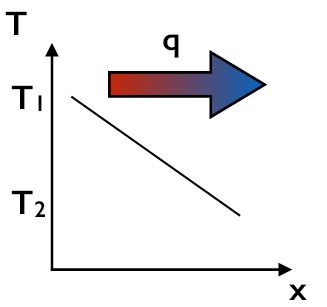
\includegraphics[scale=0.6]{./fourier.jpg}
\caption{Loi de Fourier}
\end{figure}
$k(T)$ est le coefficient de conductivité thermique et dans le cas d'un matériau anisotrope, ce n'est plus un scalaire mais bien un tenseur du deuxième ordre.
\paragraph{}
Et voilà, nous avons dérivé les lois de constitution de notre matériau ! Nous avons déterminé $\boldsymbol{\sigma}(T,\boldsymbol{\epsilon})$, $U(T,\boldsymbol{\epsilon})$, $S(T,\boldsymbol{\epsilon})$ et $\fv{q}(T)$, sous les hypothèses d'une thermoélasticité infinitésimale, linéaire et isotrope. Les inconnues sont maintenant les champs de déplacements $u(\fv{x},t)$ et de température $T(\fv{x},t)$ (nos deux variables indépendantes).
\subsection{Les équations}
En injectant les équations de constitution dans les équations de conservation, on obtient pour la conservation de la quantité de mouvement:
$$\rho_0\frac{\partial^2u_i}{\partial t^2}=\rho_0f_i-\frac{\partial}{\partial x_i}(3\kappa\alpha(T-T_0))+\frac{\partial}{\partial x_i}\left(\lambda\frac{\partial u_j}{\partial x_j}\right)+\frac{\partial}{\partial x_j}\left(\mu\left(\frac{\partial u_i}{\partial x_j}+\frac{\partial u_j}{\partial x_i}\right)\right)$$
et pour la conservation de l'énergie:
$$\rho_0c_\epsilon\frac{\partial T}{\partial t}=-3\kappa\alpha T\frac{\partial\epsilon_{mm}}{\partial t}+\rho_0\varepsilon+\frac{\partial}{\partial x_i}\left(k\frac{\partial T}{\partial x_i}\right).$$
\paragraph{}
On va cependant opérer quelques simplifications pour alléger ces expressions. La première consiste à considérer des problèmes statiques ou quasi-statiques pour lesquels les sollicitations sont lentes par rapport aux caractéristiques du matériau (la configuration s'adapte sans effet d'inertie). Cela supprime un terme:
$$\rho_0\frac{\partial^2u_i}{\partial t^2}\simeq 0.$$
La deuxième simplification est de considérer que le problème thermique est découplé du problème élastique:
$$-3\kappa\alpha T\frac{\partial \epsilon_{mm}}{\partial t}\simeq 0.$$ Le problème thermique peut donc être résolu avant le problème élastique:

$$\begin{array}{ll}
\rho_0c_\epsilon\frac{\partial T}{\partial t}=\rho_0\varepsilon+\frac{\partial}{\partial x_i}\left(k\frac{\partial T}{\partial x_i}\right)&\text{(Problème thermique)}\vspace{0.4cm}\\
\rho_0f_i=\frac{\partial}{\partial x_i}(3\kappa\alpha(T-T_0))-\frac{\partial}{\partial x_i}\left(\lambda\frac{\partial u_j}{\partial x_j}\right)-\frac{\partial}{\partial x_j}\left(\mu\left(\frac{\partial u_i}{\partial x_j}-\frac{\partial u_j}{\partial x_i}\right)\right) &\text{(Problème élastique)}
\end{array}$$

\subsection{Le problème thermique}
\subsubsection*{Données}
Afin de résoudre la partie thermique d'un problème, il nous faut:
\begin{enumerate}
\item Des conditions frontières:
	\begin{itemize}
	\item Température donnée sur une partie de la frontière, $\partial\Omega^*$:
	  $$\forall t\geq t_0,\, T=\bar{T}(\fv{x},t),\, \fv{x}\in\partial\Omega^*$$
	\item Flux de chaleur donné sur l'autre partie de la frontière, $\partial\Omega^{**}$:
	 $$\forall t\geq t_0,\, q(\fv{n})=-\fv{q}\cdot\fv{n}=\bar{q}(\fv{x},t),\, \fv{x}\in\partial\Omega^{**}$$
	\end{itemize}
\item Des conditions initiales si le problème est instationnaire: $$T(\fv{x},t_0)=T_{in}(\fv{x})$$
\item La puissance calorifique dans le volume:
$$\forall t\geq t_0,\,\rho_0\boldsymbol{\varepsilon}=\rho_0\bar{\boldsymbol{\varepsilon}}(\fv{x},t),\, \fv{x}\in \Omega.$$
\end{enumerate}
\subsubsection*{Existence et unicité de la solution}
On peut se demander si un tel problème possède toujours une solution, et si oui, est-elle unique? Pour les problèmes instationnaires, ou stationnaires avec $\partial\Omega^*\neq \emptyset$, le problème admet une et une seule solution à condition que $\Omega$, $\partial\Omega^*$, $\partial\Omega^{**}$, les CF et les CI soient suffisamment réguliers. Si le problème est stationnaire et que $\partial\Omega^*=\emptyset$, en revanche, les conditions sont plus compliquées. L'existence est assurée si
$$\oint_{\partial\Omega}\bar{q}ds+\int_{\Omega}\rho\bar{\varepsilon} \dif v=0\text{  (Conservation globale)}.$$
Si de plus la température est imposée en un point, la solution est unique.

\subsection{Le problème élastique}
\subsubsection*{Données}
Afin de résoudre la partie élastique d'un problème, il nous faut:
\begin{enumerate}
\item Des conditions frontières:
	\begin{itemize}
	\item Déplacement donné sur une partie de la frontière, $\partial\Omega'$:
	 $$\forall t\geq t_0,\, \fv{u}=\bar{\fv{u}}(\fv{x},t), \fv{x}\in\partial\Omega'$$
	\item Forces de contact données sur l'autre partie de la frontière, $\partial\Omega''$:
	 $$\forall t\geq t_0,\, \fv{t}(\fv{n})=\bar{\fv{t}}(\fv{x},t), \fv{x}\in\partial\Omega''$$
	\end{itemize}
\item Des conditions initiales si le problème est instationnaire: $$\fv{u}(\fv{x},t_0)=\fv{u}_{in}(\fv{x})\qquad \frac{\partial\fv{u}}{\partial t}(\fv{x},t_0)=\dot{\fv{u}}_{in}(\fv{x})$$
\item Les forces à distances:
\end{enumerate}
$$\forall t \geq t_0,\, \rho_0\fv{f}=\rho_0\bar{\fv{f}}(\fv{x},t),\,\fv{x}\in\Omega$$
\subsubsection*{Existence et unicité de la solution}
Les conditions d'existence et d'unicité sont similaires à celles vues dans le cas du problème thermique. Si le problème est stationnaire et si $\partial\Omega'=\emptyset$, les conditions d'existence sont alors:
$$\oint_{\partial\Omega''}\bar{\fv{t}}ds+\int_{\Omega}\rho\bar{\fv{f}} \dif v=0$$
et
$$\oint_{\partial\Omega''}\fv{x}\wedge\bar{\fv{t}}ds+\int_{\Omega}\fv{x}\wedge\rho\bar{\fv{f}} \dif v=0.$$Si de plus $\fv{u}$ et $\boldsymbol{\omega}$ sont imposés en un point, la solution est unique.
\paragraph{}
Nous possédons un système d'équations aux dérivées partielles et de conditions frontières et initiales. Il ne reste donc plus qu'à résoudre (analytiquement) le problème.

\subsection{Techniques de résolution analytique}
\subsubsection*{Le principe de Saint-Venant}
Un problème élastique aux conditions frontières requiert de connaître les déplacements ou les forces de contact en tout point de la frontière, ce qui est loin d'être une sinécure. Le principe de Saint-Venant consiste à remplacer la distribution réelle des forces de contact sur la frontière par une distribution statistiquement équivalente:
$$\int_{\Omega'}\fv{t} \dif s=\int_{\Omega'}\fv{t}' \dif s$$ La solution alors obtenue sera essentiellement la même que la solution ``réelle'' à une distance suffisamment grande de l'application de cette condition frontière (pour une poutre par exemple, une distance suffisamment grande serait deux fois la hauteur de la poutre).
\subsubsection*{La méthode semi-inverse}
La méthode semi-inverse consiste à exploiter les caractéristiques du problème pour en déduire la forme de la solution, $u_i=f_i(x_j)$. Par exemple, par symétrie certaines composantes de contraintes/déformations peuvent être supposées nulles et le champ de déplacement peut être indépendant de certaines variables. On utilise ensuite les lois de conservation et de comportement pour obtenir la solution (unique) si elle existe.
\paragraph{}
Si l'on utilise la méthode semi-inverse avec le principe de Saint-Venant, on exigera que la solution devinée reproduise des efforts statistiquement équivalents aux conditions frontières.
\subsubsection*{Principe de superposition}
Vu la linéarité de la température $T(\fv{x},t)$ par rapport aux sollicitations $\rho_0\varepsilon(\fv{x},t)$, $\bar{T}(\fv{x},t)$, $\bar{q}(\fv{x},t)$ et $T_{in}(\fv{x},t)$, si deux problèmes (1) et (2) possèdent respectivement comme solution $T^{(1)}(\fv{x},t)$ et $T^{(2)}(\fv{x},t)$, alors la combinaison linéaire $T(\fv{x},t)=\alpha T^{(1)}(\fv{x},t)+\beta T^{(2)}(\fv{x},t)$ est solution du problème ayant pour sollicitations $\alpha\rho_0\varepsilon^{(1)}+\beta\rho_0\varepsilon^{(2)}$, $\alpha\bar{q}^{(1)}+\beta\bar{q}^{(2)}$, etc.
\paragraph{}
Le principe de superposition s'applique de manière similaire au problème élastique, pour lequel $\fv{u}(\fv{x},t)$ est linéaire par rapport aux sollicitations $\rho_0\fv{f}(\fv{x},t)$, $T(\fv{x},t)$, $\bar{\fv{u}}(\fv{x},t)$, $\bar{\fv{t}}(\fv{x},t)$, $\fv{u}_{in}(\fv{x},t)$ et $\dot{\fv{u}}_{in}(\fv{x},t)$.

\section{Problèmes élastiques homogènes (cas simples)}
\subsection{Cisaillement simple isotherme}
Dans le cas d'un cisaillement simple isotherme, la seule (petite) déformation est un rapprochement angulaire. Nommons-le $\delta\phi_{12}$. Rappelons l'équation de constitution des contraintes:
$$\sigma_{ij}=2\mu\epsilon_{ij}+\lambda\epsilon_{kk}\delta_{ij}.$$ On a donc pour la contrainte de cisaillement:
$$\sigma_{12}=2\mu\epsilon_{12}.$$ De plus, en petite déformation (cfr. section \ref{défo_infinit}, $\delta\phi_{12}\equiv \gamma$): $\epsilon_{12}=\frac{\delta\phi_{12}}{2}$, d'où:
$$\delta\phi_{12}=\frac{\sigma_{12}}{\mu}$$
\begin{figure}[!h]
\centering
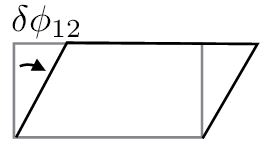
\includegraphics[scale=0.6]{./cisaillementsimplefig.jpg}
\caption{Cisaillement simple isotherme}
\label{fig:cis}
\end{figure}
\subsection{Compression simple isotherme}
En compression simple, il n'y a pas de contrainte de cisaillement et $\sigma_{ij}=-p\delta_{ij}$. Par \ref{defo-cont}, $-3p=(3\lambda+2\mu)\epsilon_{ll}$ et donc:
$$p=-\kappa\epsilon_{kk}.$$

\subsection{Dilatation simple}
En dilatation (thermique) pure (isotrope), $\sigma_{ij}=0$ et $\epsilon_{ij}=\alpha(T-T_0)\delta_{ij}$, tout simplement.
\subsection{Traction simple isotherme}
Enfin, en traction simple isotherme:
$$\epsilon_{ij}=\frac{1+\nu}{E}\sigma_{ij}-\frac{\nu}{E}\sigma_{kk}\delta_{ij} \text{ (car isotherme)}$$
$$\epsilon_{11}=\frac{\sigma_{11}}{E}$$ et
$$\epsilon_{22}=\epsilon_{33}=-\frac{\sigma_{11}}{E}$$ puisque $\sigma_{22}=\sigma_{33}=0.$

\section{Modèle du fluide visqueux newtonien}
Un fluide newtonien est un fluide pour lequel les contraintes sont linéairement proportionnelles aux gradients de vitesse.
\subsection{Principes d'un fluide visqueux}
Pour un fluide parfait, c'est-à-dire non visqueux et incompressible, ou un fluide au repos, il n'y a pas d'efforts internes autres que la pression et l'équation constitutive générale est:
$$\boldsymbol{\sigma}=-p\,\fv{I}.$$ La pression hydrostatique ($\sigma_{sph}=\frac{1}{3}\sigma_{kk}$) est alors égale à la pression thermodynamique $p$. Pour tout élément de surface, on peut calculer la force de contact $\fv{t}=\hat{\fv{n}}\cdot\boldsymbol{\sigma}=-p\,\hat{\fv{n}}$.
\paragraph{}
L'équation constitutive pour le tenseur des contraintes dans un écoulement fluide est supposé avoir la forme générale $$\boldsymbol{\sigma}=\boldsymbol{\tau}-p\,\fv{I}=\mathcal{F}(\fv{D})-p\,\fv{I},$$ où $\mathcal{F}$ est une fonction à valeur tensorielle et $\tau$ est la contrainte visqueuse. Pour rappel, \fv{D} est le tenseur des taux de déformation:
$$\fv{D}=\frac{1}{2}[\nabla\fv{v}+(\nabla\fv{v})^T].$$

\subsection{\'Equation constitutive}
On peut montrer\footnote{Cours 10 LMECA1901...} que la contrainte visqueuses $\boldsymbol{\tau}$ est
$$\tau=2\mu\fv{D}+\lambda \trace(\fv{D})\fv{I}.$$ Cela nous permet d'écrire le \emph{modèle du fluide newtonien isotrope}:
$$\boxed{\boldsymbol{\sigma}=2\mu\fv{D}+\lambda \trace(\fv{D})\fv{I}-p\,\fv{I}}$$
On peut la réécrire, en utilisant la décomposition en parties déviatoire et sphérique pour \fv{D}:
\begin{align*}
\boldsymbol{\sigma}&=2\mu(D^{sph}\fv{I}+\fv{D}^d)+\lambda \trace(\fv{D})\fv{I}-p\,\fv{I}\\
 &=2\mu\fv{D}^d+\left(\frac{2\mu}{3}+\lambda\right)\trace(\fv{D})\fv{I}-p\,\fv{I}
\end{align*}
\paragraph{Quelques remarques:}
\begin{itemize}
\item Au repos, $\fv{D}=0$ et on a bien $\boldsymbol{\sigma}=-p\,\fv{I}$
\item Ce modèle est linéaire dans les taux de déformation.
\item $\mu(p,T)$ est la \emph{viscosité dynamique de cisaillement} et est une constante de proportionnalité entre  déformation de cisaillement et contrainte.
\item Le coefficient $\frac{2}{3}\mu(p,T)+\lambda(p,T)$ est quant à lui la \emph{viscosité dynamique de dilatation}
\item La pression hydrostatique (ou pression normale moyenne), $\frac{1}{3}\trace(\boldsymbol{\sigma})$, n'est égale à la pression thermodynamique que si $\nabla\cdot\fv{v}=\trace(\fv{D})=0$ (conservation de la masse si écoulement incompressible de masse volumique constante), ou si la viscosité dynamique de dilatation est nulle.

\end{itemize}

\subsection{Compatibilité avec le second principe}
Nous allons maintenant regarder si la loi de constitution obtenue est compatible avec le second principe, dans le cas d'un écoulement incompressible\footnote{Un fluide est rarement incompressible, mais on peut souvent faire l'hypothèse que \emph{l'écoulement} est incompressible.}. Pour un tel écoulement on a $\nabla\cdot\fv{v}=\trace(\fv{D})=0$ et $\boldsymbol{\sigma}=2\mu\fv{D}-p\,\fv{I}$. Le second principe est exprimé par l'inégalité:

$$\rho T\frac{DS}{Dt}-\rho\frac{De}{Dt}\geq\frac{1}{T}\fv{q}\cdot\nabla T-\boldsymbol{\sigma}:\fv{D}.$$ Dans cette inégalité,
on a\footnote{Ici, $S=S(T)$ et $e=e(T)$.}:

\begin{align*}
\rho T\frac{DS}{Dt}&=\rho T\frac{dS}{dT}\frac{DT}{Dt}=\rho T\frac{c_v}{T}\frac{DT}{Dt};\\
\rho\frac{De}{Dt}&=\rho c_v\frac{DT}{Dt};\\
\frac{1}{T}q_i\frac{\partial T}{\partial x_i}&=-\frac{1}{T}k\frac{\partial T}{\partial x_i}\frac{\partial T}{\partial x_i};\\
\sigma_{ij}D_{ji}&=\sigma_{ij}D_{ij}=(-p\delta_{ij}+2\mu D_{ij})D_{ij}=-pD_{ii}+2\mu D_{ij}D_{ij}= 2\mu D_{ij}D_{ij} \text{ (car $D_{ii}=0$)}
\end{align*}

En insérant ces relations dans l'inégalité de Clausius-Duhem on obtient:
$$2\mu\underbrace{DijDij}_{>0}+\frac{k}{T}\underbrace{\frac{\partial T}{\partial x_i}\frac{\partial T}{\partial x_i}}_{>0}\geq 0$$
Cela nous permet de déterminer le signe de $k$ et $\mu$, car l'inéquation doit être respectée pour tout état de déformation et de température du fluide:
$$\boxed{k(T)\geq 0, \qquad \mu(p,T)\geq 0}$$

\subsection{\'Equations de Navier-Stokes}
Les équations de Navier-Stokes sont les équations de conservations de la quantité de mouvement et de l'énergie dans le cas d'un fluide visqueux newtonien (et, ici, incompressible; $\boldsymbol{\sigma}=2\mu\fv{D}-p\,\fv{I}$).
\subsubsection*{Conservation de la quantité de mouvement}
Nous pouvons insérer notre loi de comportement de $\boldsymbol{\sigma}$ dans la loi de conservation de la quantité de mouvement:
$$\rho\frac{D\fv{v}}{Dt}=\rho\fv{f}+\nabla\cdot\boldsymbol{\sigma}$$
avec $\frac{D\fv{v}}{Dt}=\frac{\partial\fv{v}}{\partial t}+\fv{v}\cdot\nabla\fv{v}$.
$$\Rightarrow\rho\left(\frac{\partial v_i}{\partial t}+v_j\frac{\partial v_i}{\partial x_j}\right)=\rho f_i-\frac{\partial p}{\partial x_i}+\frac{\partial}{\partial x_j}\left(\mu(T)\left(\frac{\partial v_i}{\partial x_j}+\frac{\partial v_j}{\partial x_i}\right)\right) $$ où $i$ est un indice libre et $j$ un indice muet (cette équation en cache donc trois). En considérant le paramètre $\mu$ constant:
$$\rho\left(\frac{\partial v_i}{\partial t}+v_j\frac{\partial v_i}{\partial x_j}\right)=\rho f_i-\frac{\partial p}{\partial x_i}+\mu\left(\frac{\partial^2v_i}{\partial x_j\partial x_j}+\underbrace{\frac{\partial^2 v_j}{\partial x_j\partial x_i}}_{\nabla(\div{\fv{v}})=0}\right) $$

$$\boxed{\rho\left(\frac{\partial v_i}{\partial t}+v_j\frac{\partial v_i}{\partial x_j}\right)=\rho f_i-\frac{\partial p}{\partial x_i}+\mu\frac{\partial^2v_i}{\partial x_j\partial x_j}} $$

\subsection*{Conservation de l'énergie}
On procède de manière similaire pour la conservation de l'énergie:
$$\rho\frac{De}{Dt}=-\nabla\cdot\fv{q}+\rho\varepsilon+\boldsymbol{\sigma}:\fv{D}.$$
On a vu plus haut que $\sigma_{ij}D_{ij}=2\mu D_{ij}D_{ij}$ (le terme $D_{ij}D_{ij}$ est un scalaire!). De plus:
$$D_{ij}=\frac{1}{2}\left[\frac{\partial v_j}{\partial x_i}+\frac{\partial v_i}{\partial x_j}\right]$$
$$\Rightarrow \rho\left(\frac{\partial e}{\partial t}+v_i\frac{\partial e}{\partial x_i}\right)=\frac{\partial}{\partial x_i}\left(k(T)\frac{\partial T}{\partial x_i}\right)+\rho\varepsilon+\frac{1}{2}\mu(T)\left(\frac{\partial v_j}{\partial x_i}+\frac{\partial v_i}{\partial x_j}\right)\left(\frac{\partial v_j}{\partial x_i}+\frac{\partial v_i}{\partial x_j}\right)$$
et comme $\frac{\partial e}{\partial t}=\frac{de}{dT}\frac{\partial T}{\partial t}=c_v(T)\frac{\partial T}{\partial t}$, et en considérant $c_v$, $\mu$ et $k$ constants:
$$\boxed{\rho c_v\left(\frac{\partial T}{\partial t}+v_i\frac{\partial T}{\partial x_i}\right)=k\frac{\partial^2 T}{\partial x_i\partial x_i}+\rho\varepsilon+\frac{1}{2}\mu\left(\frac{\partial v_j}{\partial x_i}+\frac{\partial v_i}{\partial x_j}\right)\left(\frac{\partial v_j}{\partial x_i}+\frac{\partial v_i}{\partial x_j}\right)}$$
\paragraph{}
Les deux équations de Navier-Stokes étant découplées, le problème thermique peut être résolu après le problème mécanique.
\subsubsection*{Problème mécanique: données}
Comme c'était le cas pour le problème de thermoélasticité, nous avons besoin de conditions aux frontières (et de conditions initiales) pour notre problème mécanique.
\begin{enumerate}
\item Conditions frontières:
	\begin{itemize}
	\item Vitesse donnée sur $\partial \Omega'$:
	 $$\forall t \geq t_0,\,\fv{v}=\bar{\fv{v}}(\fv{x},t),\, \fv{x}\in \partial \Omega'$$
	\item Forces de contact données sur $\partial\Omega''$:
	 $$\forall t \geq t_0,\,\fv{t}(\fv{n})=\boldsymbol{\sigma}^T\fv{n}=\bar{\fv{t}}(\fv{x},t),\, \fv{x}\in \partial \Omega''$$
	 \item Conditions mixtes: vitesse normale + forces tangentielles données, ou vitesse tangentielle + force normale.
	\end{itemize}
\item Conditions initiales, si problème instationnaire :
 $$\fv{v}(\fv{x},t)=\fv{v}_{in}(\fv{x})\qquad\nabla\cdot\fv{v}_{in}=0$$
 \item Forces à distance données sur l'ensemble de la région $\Omega$.
\end{enumerate}
\paragraph{Conditions frontières spéciales: }

\begin{enumerate}
\item Non-glissement à une paroi: $$\fv{v}=\bar{\fv{v}}(\fv{x},t)=\text{vitesse de la paroi}$$
\item Frontières libres, par exemple à l'interface avec un autre fluide visqueux libre de se déformer:
	\begin{itemize}
	\item Continuité des vitesses: $\fv{v}_{(1)}=\fv{v}_{(2)}$
	\item \'Equilibre des forces de contact: $\fv{t}_{(1)}=-\fv{t}_{(2)}$
	\end{itemize}
\end{enumerate}

\subsection{L'écoulement de Couette}
Un écoulement de Couette est un écoulement stationnaire d'un fluide visqueux incompressible entre deux plaques parallèles dont l'une est en mouvement à vitesse $U$.
Si $U=0$, on parle d'écoulement de Poiseuille.
\begin{figure}[!h]
\centering
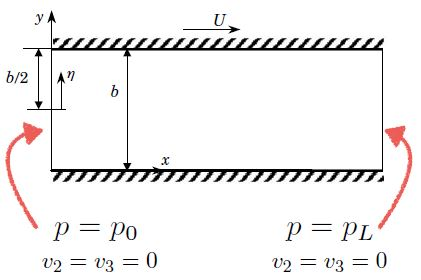
\includegraphics[scale=0.6]{./couette.jpg}
\caption{\'Ecoulement de Couette}
\label{fig:couette}
\end{figure}

\begin{figure}[!h]
\centering
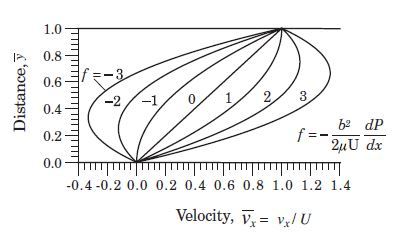
\includegraphics[scale=0.6]{./couettegraphe.jpg}
\caption{Distribution des vitesses pour un écoulement de Couette}
\label{couettegraphe}
\end{figure}

\begin{figure}[!h]
\centering
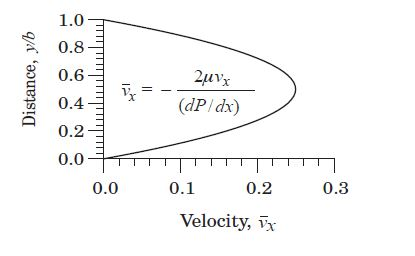
\includegraphics[scale=0.6]{./poiseuille.jpg}
\caption{Distribution des vitesses pour un écoulement de Poiseuille}
\label{fig:poiseuille}
\end{figure}

\subsection{\'Ecoulement compressible}
Dans le cas d'un écoulement incompressible, nous avons obtenu 4 équations (conservation de la masse et de la quantité de mouvement) pour les 4 inconnues $v_i$ et $p$. La pression répond donc directement à la dynamique de l'écoulement, et ce pour imposer la conservation de la masse et du volume.
\paragraph{}
Dans le cas plus général où l'écoulement est compressible, $\trace(\fv{D})\neq 0$ et on a alors les équations de conservation suivantes:
\begin{itemize}
\item Pour la masse:
	$$\frac{D\rho}{Dt}+\rho\frac{\partial v_i}{\partial x_i}=0$$
\item Pour la quantité de mouvement:
 $$\rho\left(\frac{\partial v_i}{\partial t}+v_j\frac{\partial v_i}{\partial x_j}\right)=\rho f_i+\frac{\partial}{\partial x_j}\left(-p\delta_{ij}+\mu(T)\left(\frac{\partial v_i}{\partial x_j}+\frac{\partial v_j}{\partial x_i}\right)+\lambda(T)\frac{\partial v_j}{\partial x_j}\delta_{ij}\right)$$
\item Pour l'énergie:
\begin{align*}
\rho c_v(T)\left(\frac{\partial T}{\partial t}+v_i\frac{\partial T}{\partial x_i}\right)&=\frac{\partial}{\partial x_i}\left(k(T)\frac{T}{\partial x_i}\right)+\rho\varepsilon-p\frac{\partial v_i}{\partial x_i}\\
 &+\frac{1}{2}\mu(T)\left(\frac{\partial v_i}{\partial x_j}+\frac{\partial v_j}{\partial x_i}\right)\left(\frac{\partial v_i}{\partial x_j}+\frac{\partial v_j}{\partial x_i}\right)\\
 &+\lambda(T)\left(\frac{\partial v_i}{\partial x_i}\right)^2
\end{align*}
\end{itemize}
Cela nous donne 5 équations, à laquelle on ajoute l'équation de constitution pour l'entropie et une équation d'état $\mathcal{F}(p,\rho,T)=0$. La pression est maintenant une variable thermodynamique en tant que telle.

\subsection{Forme adimensionnelle}
Replaçons-nous dans le cas d'un écoulement \emph{incompressible} du fluide visqueux newtonien, et supposons que l'écoulement soit isotherme et qu'il n'y ait pas de forces à distances. Les grandeurs du problème sont $\rho$, $V$, $L$ et $\mu$. Afin de rendre les équations adimensionnelles, nous allons effectuer les changements de variables suivants:
\begin{align*}
x_i&=Lx'_i\\
t&=\frac{L}{V}t'\\
v_i&=Vv'_i\\
p&=\rho V^2 p'
\end{align*}
Ce qui nous donne pour les équations de conservations de la masse et de Navier-Stokes:
$$\frac{\partial v_i'}{\partial x_i'}=0$$
$$\frac{\partial v_i'}{\partial t'}+v_j'\frac{\partial v_i'}{\partial x'_j}=-\frac{\partial p'}{\partial x'_i}+\frac{1}{Re}\frac{\partial^2v'_i}{\partial x'_j\partial x'_j}$$
où $Re$ est le nombre de Reynolds, qui caractérise complètement l'écoulement:
$$Re=\frac{\rho VL}{\mu}=\frac{\rho V^2}{\mu\frac{V}{L}}\sim \frac{\text{Forces d'inertie}}{\text{Forces de viscosité}}.$$ Si deux écoulements possèdent un même nombre de Reynolds (tout en pouvant avoir des variables $\rho$, $V$, $L$ et $\mu$ différentes), alors la solution (adimensionnelle) du problème est la même pour les deux écoulements, à une mise à l'échelle près.
\paragraph{}
Un nombre de Reynolds faible traduit une dominance des forces visqueuses et est caractéristique d'un écoulement stationnaire.  \`A l'inverse, un $Re$ élevé montre que les forces d'inertie croissent et peuvent mener à des instabilités et des écoulements instationnaires.

\section{\'Ecoulement d'un fluide parfait}
Un fluide parfait est un fluide non visqueux et donc caractérisé par un nombre de Reynolds infiniment grand: $Re\rightarrow \infty \sim \mu=0 \text{ et } \sigma_{ij}=-p\delta_{ij}$.
$$\rightarrow\frac{\partial v'_i}{\partial t'}+v'_j\frac{\partial v'_i}{\partial x'_j}=-\frac{\partial p'}{\partial x'_i}$$
En retournant en dimensionnel, on obtient les \emph{équations d'Euler}:
$$\frac{\partial v_i}{\partial x_i}=0$$
$$\rho\left(\frac{\partial v_i}{\partial t}+v_j\frac{\partial v_i}{\partial x_j}\right)=-\frac{\partial p}{\partial x_i}$$ Nous avons donc une forme asymptotique des équations de conservation de la masse et de Navier-Stokes, valable pour un fluide parfait ou loin des parois où les effets visqueux sont faibles.
\paragraph{}
Pour dériver les équations d'Euler, on a modifié l'ordre de l'équation de Navier-Stokes: initialement d'ordre 2, on est passé à l'ordre 1. Les conditions limites doivent donc être modifiées en conséquence. On ne peut plus imposer la vitesse de la paroi, à la place on va imposer le glissement à la paroi: $$\fv{v}\cdot\hat{\fv{n}}=\bar{v}_n(\fv{x},t)$$
Près des parois, le terme du deuxième ordre $\mu\frac{\partial^2v_i}{\partial x_j\partial x_j}$ n'est plus négligeable, les équations d'Euler ne sont donc plus valables. Connaître la zone où le terme visqueux devient non négligeable est un problème de couche-limite.

\section{Discontinuités}
Que se passe-t-il si des discontinuités apparaissent dans notre milieu continu? Comment gérer les irrégularités locales comme l'interface entre 2 fluides, un choc dans un écoulement compressible, un front de solidification?
\paragraph{}
Pour prendre en compte ces discontinuités, on va considérer un volume de contrôle $\Omega$ assez petit sur une surface $\Sigma(t)$ qui bouge avec une vitesse normale $v^*_n$. Le volume de contrôle suit l'interface avec une vitesse $v^*_n$. On pourra ensuite appliquer la relation \ref{comparaison_mat_cont}.
\paragraph{Relation pour la masse}
L'application de la relation \ref{comparaison_mat_cont} à la fonction $\phi(\fv{x},t)=\rho(\fv{x},t)$ (densité) pour un volume de contrôle de vitesse $v^*_n\hat{\fv{n}}$ (voir figure \ref{fig:disc_vol_cont}) donne:
$$\fdif{}{t}\int_{\Omega (t)}\rho  \dif v=\frac{D}{Dt}\int_{\Omega (t)}\rho  \dif v+\oint_{\partial \Omega (t)}\rho(\fv{v}_s-\fv{v})\cdot \fv{\^n}' \dif s$$
où $\hat{\fv{n}}'$ est la normale courante et vaut $\hat{\fv{n}}_1=-\hat{\fv{n}}$ et $\hat{\fv{n}}_2=\hat{\fv{n}}$ sur les bases du cylindre, si notre volume de contrôle est un cylindre de longueur $\epsilon$ dont les bases ont un rayon $R$ et une surface $S$ et dont l'axe est dans la direction de $\hat{\fv{n}}$.
Par conservation de la masse, le premier terme à droite de l'égalité est nul. S:
\begin{align*}
\fdif{}{t}\int_{-\epsilon/2}^{\epsilon/2}\int_{S_{tot}} \rho \dif xds=&\int_{S_2}\rho_2(v_n^*\hat{\fv{n}}-\fv{v})\cdot\hat{\fv{n}}_2 \dif s\\
 &+\int_{S_1}\rho_1(v_n^*\hat{\fv{n}}-\fv{v})\cdot\hat{\fv{n}}_1 \dif s\\
 &+\int_{-\epsilon/2}^{\epsilon/2}\int_0^{2\pi}\rho(v_n^*\hat{\fv{n}}-\fv{v})\cdot\hat{\fv{n}}'R \dif \theta  \dif x
\end{align*}
En faisant tendre $\epsilon$ vers 0, il reste ($S_1=S_2=S$):
$$\int_{S}\rho_2(v_n^*\hat{\fv{n}}-\fv{v})\cdot\hat{\fv{n}}-\rho_1(v_n^*\hat{\fv{n}}-\fv{v})\cdot\hat{\fv{n}} \dif s=0$$
\begin{figure}[!h]
\centering
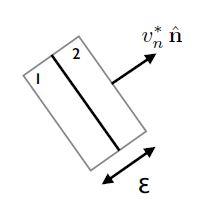
\includegraphics[scale=0.6]{./discontinuite_vol_controle.jpg}
\caption{Volume de contrôle}
\label{fig:disc_vol_cont}
\end{figure}
On a ainsi montré que dans le cas d'une discontinuité entre 1 et 2, on a la relation\footnote{On utilise la notation $[\cdot]=(\cdot)_2-(\cdot)_1$}:
$$\boxed{[\rho(\fv{v}^*-\fv{v})\cdot\hat{\fv{n}}]=0}$$
\paragraph{Relation pour la quantité de mouvement}
Utilisons le même raisonnement avec la fonction $\boldsymbol{\phi}=\rho\fv{v}$ (quantité de mouvement). La relation \ref{comparaison_mat_cont} devient:
$$\underbrace{\fdif{}{t}\int_{\Omega (t)}\rho\fv{v}  \dif v}_{\rightarrow 0}=\frac{D}{Dt}\int_{\Omega (t)}\rho\fv{v}  \dif v+\oint_{\partial \Omega (t)}\rho\fv{v}(v_n^*\hat{\fv{n}}-\fv{v})\cdot \hat{\fv{n}}' \dif s$$
Par conservation de la quantité de mouvement:
$$\frac{D}{Dt}\int_{\Omega (t)}\rho\fv{v}  \dif v = \underbrace{\int_{\Omega}\rho\fv{f} \dif v}_{\rightarrow 0}+\oint_{\partial\Omega}\fv{t}(\hat{\fv{n}}') \dif s$$
d'où:
\begin{align*}
0=&\int_{S_2}\fv{t}(\hat{\fv{n}}_2) \dif s + \int_{S_1}\fv{t}(\hat{\fv{n}}_1) \dif s + \underbrace{\int_{-\epsilon/2}^{\epsilon/2}\int_0^{2\pi}R\fv{t} (\hat{\fv{n}}') \dif xd\theta}_{\rightarrow 0}\\
 &+\int_{S_2}\rho_2\fv{v}_2(v_n^*\hat{\fv{n}}-\fv{v})\cdot\hat{\fv{n}}_2 \dif s + \int_{S_1}\rho_1\fv{v}_1(v_n^*\hat{\fv{n}}-\fv{v})\cdot\hat{\fv{n}}_1 \dif s
\end{align*}
Et comme $\hat{\fv{n}}_1=-\hat{\fv{n}}$, $\hat{\fv{n}}_2=\hat{\fv{n}}$ et $\fv{t}(-\hat{\fv{n}})=-\fv{t}(\hat{\fv{n}})$, on arrive à la relation:
$$\boxed{[\rho\fv{v}(\fv{v}^*-\fv{v})\cdot\hat{\fv{n}}+\fv{t}(\hat{\fv{n}})]=0}$$

\paragraph{Relation pour l'énergie}
On peut de la même manière trouver une relation pour l'énergie dans le cas d'une discontinuité entre 1 et 2:
$$\left[\rho\left(e+\frac{1}{2}\fv{v}\cdot\fv{v}\right)(\fv{v}^*-\fv{v})\cdot\hat{\fv{n}}+\fv{t}(\hat{\fv{n}})\cdot\fv{v}+h(\hat{\fv{n}})\right]=0.$$
\paragraph{}
\vspace{3cm}



\appendix
\part{Annexes}
\section{Problème de Stefan (Tuyau CM11)}
Le probleme de Stefan est qu'on a un bloc de glace à une certaine température, on voudrait savoir comment faire le lien entre le déplacement de la glace (de l'interface glace/air) et le flux de chaleur.

On a donc un flux de chaleur qui passe de l'air à la glace, qui fait changer la température de la glace à l'interface, donc elle va fondre et déplacer l'interface.

Ce qui est tuyaux je pense c'est de savoir résoudre ce problème pour $T_g$ et $T_a$ (température dans la glace et dans l'air, représentées par la courbe sur le slide). On doit utiliser la conservation de quantité de mouvement pour résoudre ce problème. (Voir deux dernies slides du CM11)
La page Wikipedia sur le sujet explique bien le problème: \url{https://en.wikipedia.org/wiki/Stefan_problem}
Voir aussi des notes manuscrites (à recopier joliment ici): \url{http://www.forum-epl.be/viewtopic.php?t=12453}.

\end{document}
